
\section{IMPLEMENTATION: Relating the market model to the code}
The chapter links the theory to the output of the simulations. %is intended to explain the code and justify the modeling decisions that link the theory to the actual 


\section{MOVE UP? Bargaining - The market process and bargaining}
We consider a homogeneous city with a single wage, identical preferences, uniform identical transportation costs, identical lot sizes.

Individuals and institutions buy and sell properties given individual goals, resources and available information.

% The process can be summarized as
The model of the market process includes the following steps:
The core machinery of the model is the market process. At the centre of that process is a model of price formation and bargaining. % bargaining model. 

\begin{enumerate}
    \item Identify the set of sellers for the current cycle. This may include:
    \begin{enumerate}
        \item people retiring in this cycle,
        \item people who retired and failed to sell, and potentially
        \item people approaching retirement who might consider selling early and
        \item financialized owners. % the bank? speculative owners? .
    \end{enumerate}
    
    \item For each seller, calculate the expected property price: % \textbf{from real estate agent}:
    \begin{enumerate}
        \item Initialize with the warranted price, which is the value of the stream of services, provided by the property. Rents minus net costs:
       \[ P_W=\frac{(\omega-{dc}) + {a}\psi}{r}\]
        The value of the house is the rent premium minus the cost of transportation. Subtract the costs of running the house, divided by the interest rate
    
        IS IT MINUS A $\psi$ SINCE HIGHER COSTS LOWER PRICES?
       
        {\color{green} This is the expected warranted price. It might make sense just to use the homeowner's reservation price (maximum bid price)}.
        \item in later cycles use the actual transaction price $P_M$ (with inflation added) when it is available, or use a (regression)estimate $P_{it}^e$ the real estate agent.
    \end{enumerate}
    
    \item for each seller, compute a reservation price using a variant of the maximum bid price formula. 
    {\color{green}\textit{Values like $m_i$ are going to be expected values for others.  ??? }}
    \textit{This is what the seller thinks she should get, taking into account her expectations about the price increase etc..}
    
    \item for each seller, compute an asking price. 
    \textit{Add some percentage to the reservation price. Make sure the result is above ***? $P_M^e$, since you know you might have to come down in bargaining.}   
    
    \item for each seller, list the asking price for bidders to see.
    
    \item for each property, identify a set of potential bidders.
    \begin{enumerate}
        \item Bank considers bidding on all listed properties.
        the formula is the maximum bid price with its own parameters putting in the current rents.
        \item New entrants to labour market
       {\color{yellow} \item Retirees who might sell, move out of town and invest in a rental property}
    \end{enumerate}
    
    \item for each bidder, compute a maximum price using a variant of the bid price formula. 
    
    \item for each bidder, compute an initial bid no higher than  the maximum price. 
    \color{red}  
    \textbf{(there may be two paths to consider: working from initial bids, or working with max bids )}
    
    \item With list of max bids, check to see if any exceed the asking price. 
    \begin{enumerate}
        \item If yes settle on asking price if there is just one, and the second highest max bid if there are more than one.
        \item If no, proceed.
    \end{enumerate}
    
    \item With list of max bids, check to see if any exceed the reservation price. 
    \begin{enumerate}
        \item If no, house is not sold, and reservation price is reduced for the next cycle.
        \item if one max exceeds the reservation price,  split the difference between the reservation price and the maximum bid bid.
        \item if more than one max exceeds the reservation price, choose the second highest max bid if there are more than one
    \end{enumerate} 
\end{enumerate} \color{black}


-----

All agents have access to the price forecast, $P_M^e$, from the real estate agent.

We have five categories of potential buyers.\footnote{Types three and four  would  become landlords if the transaction is completed, which is a change of class status.} 
\begin{enumerate}
    \item newcomers to the city, who have a job offer  and seek to buy a home or become tenants.  
    \item financial investors who possess financial capital and seek a rate of return better than they would receive from alternative investments. We refer to this investor as `the bank'
    \item owner-occupiers who might mortgage their current homes  to purchase a revenue property
    \item owner-workers who retire and might  invest in a revenue property rather than spending  their capital gain 
    \item sellers are also default buyers, since they can buy their own home and rent it out if their \gls{reservation price} is not met.  
\end{enumerate}


For potential sellers the maximum bid price is also the `\gls{reservation price}' price.  
\[P^{ask}> P^r, \qquad   P^{offer}< P^{max}\]


All potential buyers and potential sellers  will calculate a \gls{maximum bid price} or reservation price and and an initial offer price or ask price \gls{bid  price}. 

The initial bid price (offer) will be lower than the potential buyers maximum bid price. The initial ask price will be higher than the reservation price.

Bargaining will occur when the maximum bid price of at least one agent exceeds the reservation price of the listing agent.

Transactions can occur when the maximum bid price of at least one agent exceeds the reservation price of the listing agent.


\subsection{Determining initial offer and ask prices}

Agents can calculate their maximum bid  or their  reservation price. 
These values are not public. We need to identify initial ask and offer prices, which is the way they appear in the market.


\[P^{ask}> P^r> P_M^e\] 

If the posted expected price exceeds their \gls{reservation price} they 
\begin{enumerate}
    \item list  the property for sale with the real estate age,nt.
    \item select an asking price   
\end{enumerate}

The bank posts a \gls{maximum bid function} with the real estate agent.

In practice, potential investors will make an  initial  bid that is lower than this value and subsequent bargaining will settle of a price between the initial bid and the seller's asking price.

In the market, the initial bid should be smaller than the bid price calculated, which is a maximum that can earn the target rate of return, The bank will definitely go this high. 

% If there is a  max bid among competing buyers, the second highest max bid should be the sale price, but the bidder with the highest max bid wins the property. This is realistic because in a bidding war the final bid only has to be a very small amount higher than that of the last competitor left.
% That is the highest price that a seller can get.

 %This  seems realistic enough and is very simple to implement. It should producer a path that is indistinguishable form any more complex approach. 

% Will persons retiring who would leave the city invest in an urban rental?



% But what is $D$? Does the bank have unlimited funds? Isn't D just a fraction of P?  If so it cancels out
% r is the prime rate- that the bank pays? 



% \begin{verbatim}
% \end{verbatim}

\section{Computing values for bid and warranted price}

In the following sections we discuss % the computation of agents' bid price, outline potential discounting approaches, and discussing 
how each component of the calculation is treated in the code. %, organizing the discussion following Equation~\ref{eqn-bid-price2}:


\begin{align}
P_i^{bid} \le   \frac{\mathcal{R}_N}{(1-m_i)r_i^{target}- \delta_i \left(1+L(P)- (1+ r_i)m_i\right)}.
\end{align}
Net rent, $\mathcal{R}_N$, is discussed in section \ref{SS:NetRent}. 

Interest rates, discount rates, and borrowing ratios are discussed in section \ref{SS:RatesAndRatios},
The borrowing ratio, $m_i$, is discussed in section \ref{SS:BorrowingRatio}, the target interest rate, $r_i^{target}$, is discussed in \ref{SS:targetr} the discount factor, $\delta_i$ is discussed in section \ref{SS:discountfactor}. The price approximation mechanism, $L(P)$ is discussed in \ref{SS:PriceForecast}, and the interest rate the buyer has to pay for the mortgage, $r_i$, is discussed in \ref{SS:BankRate}. Sections are thus numbered: 

\begin{align*}
P_i^{bid} \ge   \frac{\ref{SS:NetRent}} {(1-\ref{SS:BorrowingRatio})\ref{SS:targetr}-
\left[ \ref{SS:discountfactor}(1+\ref{SS:PriceForecast}- (1+\ref{SS:BankRate})\ref{SS:YWealthConstraint})\right]}. 
\end{align*}


\section{CODE DISCUSSION}
present value of tax on propriety over T years. 

\section{Operating cost calculations}
\begin{verbatim}
property value * tau * (sum_(1-T) ((1/(1+r))^t).    
    (sum_(1-T) ((delta_t)

psi   = 100000 # subsistence wage
    
#  Annual operating cost in dollars  
#  eg psi=100000 b=.02 , a*b*psi= 2000 per year 

 compounded for 5 years Must add the discount factors  
 \delta_t for five years 
 \[ oppcost=  \[\frac{\omega+a\phi}{r} \tau + a\phi b\right]\sum_1^T \frac{1}{1+r}\]
 a*b*psi/.r - (a*b*psi/r)*delta_T
#  eg   2000/.r - (2000/r)*delta_T 
= 2000/0.05 - (2000/0/05)*delta_T = 8658.953

opperating_cost = a*b*psi/r - (a*b*psi/r)*delta_T 
\end{verbatim}

\[ oppcost=  \left(\tau\omega  +(\tau+b)a\psi\right)\sum_1^T \left(\frac{1}{1+r}\right)^t\]

\begin{verbatim}
    opperating_cost = (tau*(omega-c*d) + (tau+b) *a*psi)* sum((1/r)^t for t in range(1, T))
    
This is (tax on rent plus both tax and maintenance on the house and land) for (T years with discounting for each year),
\end{verbatim}



----


The relationship between income and consumption is suppressed, because that makes xyz.. so much clearer.

because it ignores
but the relationship

but the relation ship between x and y is not..

don't care what they do in retirement, so ignoring it, so they're still capturing capital gains so long as they own a house
t
their lifetime income is changing even though their current income is not.

--
renters get none of that.



$delta_T$ 
$sum_delta_T$
% $sum_r_T$

$r_T$  present value of total interest payments made over period T




${a}$  =  share of subsistence wage  used for land and building e.g. 0.3

${b}$  = share of share of subsistence wage  used on maintenance e.g. 0.2

${c}$  = annual tax rate on rent and home  e.g. 12 mills 


a     share of subsistence wage  used for land and building

b      share of share of subsistence wage used for maintaining home

c    annual tax rate on rent and home  eg  1.6\% = 16 mills, 1.2\% =.12 mills

% Sigma is tax share, what is the tax rate.
% delta is density ** - - infinitesmal density increase as the city moves out. [[adjustment speed for wage N]] imagine a density function over the city. 

\section{SORT Housing services 30 percent}
MOVE TO ASSUMPTIONS - We assume households spend a fixed fraction $a$ of their subsistence wage $\psi$ on housing. 

\footnote{***JUSTIFY ASSUMPTION OF FIXED SHARE OF SUBSISTENCE HERE? This appears to be empirically justified and simplifies the model \cite{GET_SOURCE_HOUSING_A_FIXED_SHARE_SUBSISTENCE_WAGE}. Appendix \ref{appendix-future-work} considers how the assumption may be relaxed in future work.}

Housing services absorb about 30\% of income  we will use than number  as an approximation,  $a\psi$, where $a$ is the share of the subsistence wage and $\psi$

Note, this is a simplification. It ignores any locational values of the house, as well as the costs stream, it is a net cost, but a net cost embedded in the share of the income. It is a justified simplification, but an interesting place to explore the effect of adding nuance.  MAYBE MOVE DISCUSSION OF POTENTIAL EXTENSIONS TO FUTURE WORK.

\section{Net rent}\label{SS:NetRent}
We assume that the present value of the rent % $\mathcal{R}$ 
is known to an investor in advance. We can imagine the investors' accountant having information on the rent that the market will bear or on prior rents and including this information in the calculation of $P_B$.

Uncertainty can be represented as bias or stochasticity.
Calculation notes: I have rent from the wages. I have kappa and sigma from our ex parameter values. . omega from the wages. 

Net rent, which can be written a share, $\phi$ of total rent $\mathcal{R}_N = \phi \mathcal{R}$
$\mathcal{R}_N = \phi \mathcal{R}$

Where the \gls{rent share}, phi is a fraction
$\phi = (rent-taxes-costs) /rent$ 

There's a distinction between the warranted rent, the net rent, and the rent that's actually charged.

We assume that the  rent  actually charged to a tenant is the warranted economic rent, ($\mathcal{R}= \omega - {dc}$), but the relevant term to enter into the calculation of return on investment is the net rent $\mathcal{R}_N$ for a given property, because the returns are the returns an investor can get after paying taxes and operating costs.

In our computational model, we do the calculation in terms of a mortgage, so we want the total returns after expenses, in present value, compounded over the mortgage  period.
% We want the total returns after expenses, in present value, compounded over a 5 year period.

\begin{align}
\mathcal{R}_N &= \mathcal{R} - \mathcal{O} - \mathcal{T} 
\end{align}

In terms of the warranted rent, 
\begin{align}
\mathcal{R}_N &= (1-\kappa_j - \sigma_j)(\omega - {dc}) % was {d_j} here
\end{align}


% $\mathcal{R}_N = (1-\kappa_j - \sigma_j) (\omega - {c} d_j)$

% {\color{red}
% Notice that  we need here is really the fraction of the warranted rent that the owner gets to keep after maintenance costs and taxes. It is possible that the owner is charging more or less than the economic  rent, but economic rent can be seen as an equilibrium value. Economic rent is $\mathcal{R}$.  This is (tautologically) related to the price as a fraction of the actual sale price: COULD MOVE TO THE CHAPTER NOW SINCE THE THE SECTION IS MOVED THER
% }
% \[\mathcal{R}= \frac{\mathcal{R}}{P_0}P_0 \]

If we want to know the  present value  of the \textbf{net rent}, $\mathcal{R}_N$  collect over the period  $T$, $\mathcal{R}_N^T$, we \textbf{add up} the discounted rents for each year. We may assume the rents are rising at and that the first is the current warranted rent, which gives us a computational formula. 
\[\mathcal{R}_N^T= (\omega-dc)\sum_{t=0}^{t=T-1} \frac{(1+\dot{\mathcal{R}})^{t}} {(1+r_{r_\delta})^{t+1}} \]

% \[\mathcal{R}_Nj^T= (\omega-dc_j)\sum_{\tau=0}^{\tau=T-1}\left[\frac{1+\dot{\mathcal{R}}}{1+r_{r_\delta}}\right]^\tau \]
\noindent where $\dot{\mathcal{R}}$ is an expected rate of change of rents - possibly zero for now, and $r_\delta$ is the individual's discount rate. 

TODO: problem - how to handle subscripts with net rent $\mathcal{R}_N$


\subsection{Tax ratio}\label{SS:TaxRatio} 
The tax ratio $\sigma$ is the share of rents that the municipality takes for services and infrastructure. This fraction of the value of the property is about 30\% based on mill rates in Ontario,  so $\sigma = 0.3$. % REFERENCE

*** CHECK Total taxes paid on  property $j$, over a given mortgage period $T$ is 

\[\Psi_j^T = \psi * \mathcal{R}\].  

    %\href{https://www.google.com/url?sa=t&rct=j&q=&esrc=s&source=web&cd=&ved=2ahUKEwiOmNPUvIL9AhUUmokEHX-5C9oQFnoECBIQAQ&url=https%3A%2F%2Fwww.greatersudbury.ca%2Fcity-hall%2Ftax-services%2Fpdf-documents%2F2022-tax-rates%2F&usg=AOvVaw2XEdfcC5z-5AqfOeH5t-eN}{Sudbury values}  same as https://www.greatersudbury.ca/city-hall/tax-services/pdf-documents/2022-tax-rates/

\subsection{Cost tax ratio}\label{SS:CostRatio} 
The value of $\kappa$  varies for every property based on maintenance requirements, historic rents, tenant rights, and variations in assessed values. If it varies, it may be useful as a quality indicator.

%Values for $\kappa$ and $\sigma$ must be adjusted to take into account the length of the period or net rents have to be summed over the period.  NO LONGER NEEDED 

Nothing prevents $\sigma+\kappa >1$, which would leave an investor unable to cover building maintenance and taxes out of current rent. 


% image.png

% image.png
% https://www150.statcan.gc.ca/n1/pub/46-28-0001/2023001/article/00001-eng.htm

% Investors now make up more than 25\% of Ontario homebuyers, pushing prices higher, experts warn. 2020

% Released: 2022-04-12

% New data from the Canadian Housing Statistics Program (CHSP) show the extent of inequalities in housing: multiple-property owners possess nearly one-third of all residential properties and the top 10\% wealthiest owners account for around one-quarter of residential housing value. Despite these inequalities, new data show an increase in the number of first-time home buyers from 2018 to 2019.
% Both income and housing wealth are concentrated at the top, even among owners. When ordering individual owners by their yearly incomes, the top 10% of owners in Ontario and British Columbia each had yearly incomes above $125,000.
 

\subsection{Borrowing ratio} \label{SS:BorrowingRatio}


The borrowing ratio, $m_i$, is just the fraction of the price that the bank will lend to a potential buyer. \textbf{It may depend on the individual.} 

Income(\ref{SS:YWealthConstraint}) and/or wealth (\ref {SS:MWealthConstraint}) may constrain individual participation in markets. 
Here we should use the same logic as we use about the interest rate charged. (\ref{SS:BorowingRate})

It is likely to be higher for institutional buyers  and for the wealthy because the bank thinks those with assets are more secure risks. they may have other assets that could be attached in the case of default.
(note interventions with reduces interest rates, or loan assessments drawing on techniques used by foundations could have value)


\subsection{Target interest rate}\label{SS:targetr}

 The target interest rate, $r^{target}$, is the prime rate plus a margin. % required by the bank.  Question: do non-bank actors have such a term?

\begin{verbatim}
self.get-target-interest-rate(buyer)
\end{verbatim}



\subsection{Discount factor}\label{SS:discountfactor}

The discount factor $\delta_i$ for THE END OF period $T$ captures the cost of waiting $T$ periods to sell the property. The usual way to treat it, which we use here, is to assume that $i$ has an interest rate $r_i$ and has been investing efficiently. This means that  the individual has a discount factor for future returns based on the year-over-year rate of return. 

\[\delta^T_i=\left[\frac{1}{1+r_i}\right]^T\]




If we want the compounded interest rate person $i$ the term T,
\[r_i^T=(1+r_i)^T\]
% This is the value we use in equation~\ref{EqBidPrice}.

If person $i$  discounts at a discount rate $r^\delta$, the present value of a receipt at time $t$ is calculated by using the \textbf{discount factor} $\delta_i^T$.

\[\delta_i^T= \left( \frac{1}{1+r_\delta} \right)^T \]
%\[\delta_i^T= \sum_{\tau=0}^{\tau=T}\left( \frac{1}{1+r_\delta} \right)^\tau \]
 
These can be combined into a function %\delta that  gives a single discounting factor  for a value  like future price that is both growing and being discounted over several (T) periods:
\[ PDV(P_M^{Te})=P_0\left( \frac{1+\dot P}{1+r_\delta} \right)^T \]
This PDV function specifically combines any expected rent increase, the individual's discount rate and the mortgage term into a single operation.

% \subsection{Mortgage availability}
% For home loans, many personal finance experts recommend total housing costs account for less than 28\% of your \textbf{gross} household income, This gives us an \textbf{income-based  mortgage maximum} of \[M^{max}_Yi = \frac{0.28*(\omega+w)}{r_i}\] It is the maximum the bank will let you pay.

% We assume $r_i$ is based on the individual's assets, on relative wealth. Where is it calculated for the householder or the bank?

% We get a \textbf{price-based mortgage maximum} \[M^{max}_P = 0.8P_0\] where $P_0$ is the actual sale price. This is based on the maximum amount of risk that the bank is willing to take on. ($P_0$  will not always be the same as the asking price or the warranted price.)

\subsection{SORT Cobb-Douglas constant fraction of income on housing}
It is convenient in this model to use a \gls{Cobb-Douglas} utility function that has the property that a fixed fraction of income is spent on housing.  We can start with the assumption that earnings are fixed for the lifetime at the one-period wage, $w$. Then total spending on housing is $\beta Y, \beta <1$ and $ Y=w$. Let the transportation cost for a specific location $l$ be $T(l)$. The  equilibrium price at that location will be $P(l)= \beta Y-T(l)$.

\section{SORT: Miscellaneous calculations about rates over time}
$delta(0)=1$  for funds received now

Lets calculate $S$, $\delta$ at time infinity:
*** Why?

\[\delta(t)=\left(\frac{1}{1+r}\right)^t\]

\begin{align}
delta (1)   &= 1/(1+r) \\
delta (t)   &= (1/(1+r))^t \\
delta (\infty)   &= \sum_0^\infty\left(1/(1+r)\right)^t\\ 
Let\ a=1/(1+r)&<1\\
delta (\infty)   &= \sum_0^\infty a^t\\ 
S               &= \sum_0^\infty a^t\\ 
               &= 1+a+a^2+a^3+a^4 \dots\\ 
S-aS             &= 1\\ 
S             &= 1/(1-a)\\ 
S             &= \frac{1}{1-\frac{1}{1+r}}\\ % subing r back in for a 
             &= \frac{1}{1-\frac{1}{1+r}}\\ 
             &= \frac{1}{\frac{1+r-1}{1+r}}\\ 
              &= \frac{1}{\frac{r}{1+r}}\\ 
             &= \frac{1+r}{r}
\end{align}
This is the case where you get paid at the beginning of the first period. Rent might be paid in advance for each month. .

For  the case where you get pay at the end of the first period. Interest on a loan  might be paid this way.  summing from t=1 this time, we get $S-aS =a$, and $S = a/(1-a)= \frac{1}{r}$. 

 

%\[\delta(t)= \delta(1)^t =\left(\frac{1}{1+r}\right)^t\]

Finally, we need an expression for the sum of a finite  series to T.  Doing the derivation to check my logic, notice that  omega, psi, c  and a are constants that can be factored out in the following,(\textbf{THIS IS THE WRONG PROPERTY VALUE}
%\[\left(c*\omega + c*a*\psi \right) ->c\left(\omega-trans\ d + a\psi \right)\]
\begin{align}%
    tax&= \sum_{t=0}^{T-1} \delta(t) \left(c*\omega + c*a*\psi \right)\\
        &= c(\omega + a\psi)\sum_{t=0}^T  \delta_t\\
        &= c(\omega + a\psi)(\delta_1+\delta_2 \dots \delta_T)\\
        &= c(\omega + a\psi) \left(\sum_0^\infty \delta_t-\sum_{T}^\infty \delta_t\right)\\
        &= c(\omega + a\psi) \left(\frac{1+r}{r}  - \left(\frac{1}{1+r}\right)^{T+1} \left(\frac{1+r}{r} \right) \right)\\
        &= c(\omega + a\psi) \frac{1+r}{r}\left(1  - \left(\frac{1}{1+r}\right)^{T+1} \right)
%      &=& c(\omega + a\psi)\delta_T\\
\end{align}

\chapter{MODEL PARTS CUT FROM BACKGROUND CHAPTERS}

\section{GROWTH}

\section{Equilibrium city size and the scale factor} 
At this point, we can briefly describe how the discussion of this chapter relates to our overall modeling. There are four basic equations in the model. The first two link output and the wage to population. the third links the wage to the extent of the city and the last  provides the population of the city

Equation one, following Bettencourt (p65) says that  urban productivity is proportional to population via a scale factor:\footnote{ In contemporary US cities productivity increases by about 11\% with each doubling of their population.  Urban Scaling and the Production Function for Cities Lobo J, Bettencourt LMA, Strumsky D, West GB (2013) PLOS ONE 8(3): e58407. https://doi.org/10.1371/journal.pone.0058407 }, 
\[Y= GN^{\beta}\]  

and has both theoretical and empirical support. 


\cite{arvidssonUrbanScalingLaws2023} find that cities' tails are responsible for 36--80\% of the observed superlinearities across indicators. 

% \begin{tabular}{ll}
% $Y$ is &Aggregate urban output, or GDP \\
% %$\alpha$ & agricultural wage\\
% $G$ is&a `prefactor,' possibly time dependent, an initial population\\
%  $N$ is& city population\\
% $ \beta$  is& scale factor, the elasticity of output with respect to city population .\\
% \end{tabular}\vspace{.5cm}

This is illustrated in Figure~\ref{fig-scale-output} for $\beta=1.25$ and $G=1$. The significant features are the upward-bending total output curve that indicates increasing productivity per capita for the city and the rising marginal product of labour.

\begin{figure}[htb]
    \begin{center}
    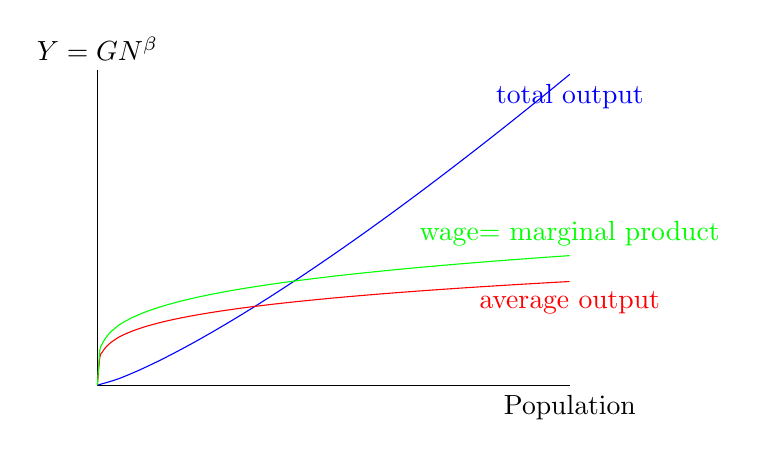
\begin{tikzpicture}
      \draw (0,4)node[above]{$Y= GN^{\beta}$}--(0,0) --(6,0)node[below]{Population};
       \draw[scale=1, domain=0:6, smooth, variable=\x, blue] plot ({\x}, {(\x/2)^1.25})node[below]{total output };% divide by 2 to get it on the plot
       %\draw (0,1)node[left]{$\alpha$}--(6,3.5)node[left]{$\alpha +\rho P$};
      \draw[scale=1, samples=200,domain=0:6, smooth, variable=\x, red] plot ({\x}, {(\x/2)^.25})node[below]{average output};% THis is the wage plot
    \draw[scale=1, samples=200,domain=0:6, smooth, variable=\x, green] plot ({\x}, {(1.25*(\x/2)^.25)})node[above]{wage= marginal product};
%[red] plot[samples=200, domain=-0:6] function {(\x/2)^.25}node[above]{wage};
      %  \node [left] at (0,2){$w=\rho P$};
         % \draw [dashed](0,3)node[left]{$Y_i$}--(6,3);
    \end{tikzpicture}\vspace{.5cm}
    \caption{Urban productivity is proportional to population, $\beta=1.13$}
    \label{fig-scale-output}
    \end{center}
\end{figure}

The right hand side of second equation is derived from the first bvy differentiation and combined with a result from the theory of the firm that says that the firm should hire until the marginal value product of labour is equal to the total wage, $\omega+w$, where $w$ is the `subsistance wage' that is earned by non-urban workers.  
\[\omega+w = \beta GN^{\beta-1}\]

The third is the population equilibrium condition, that requires that at the boundary of the city, $d^*$,  transportation costs, $td^*$, consume the entire wage:
 \[d^*=\frac{\omega}{t}\]

 The fourth is the function that generates the total urban poulation. In the standard circular city, for example, with a uniform density, $\delta$,  
 \[N=\delta\pi (d^*)^2\]
 % \[N=\delta\pi (\frac{\omega}{t})^2\]
 %\[N=\delta\pi (\frac{\beta GN^{\beta-1}-w}{t})^2\]
 
 The equilibrium population  is: 
% \[N=\delta\pi (\frac{\beta GN^{\beta-1}-w}{t})^2\]

\begin{eqnarray}
    N&=&\delta\pi (\frac{\beta GN^{\beta-1}-w}{t})^2\\
    &=&\frac{\delta\pi }{t^2} \left[\beta GN^{2\beta-2} -w^2\right]
\end{eqnarray}

This expression can be treated as a difference equation if we consider the left hand side as $M_{c}$ and the right hand side  function of the previous period's as population, $N_{{c}-1}$.



\subsection{Incorporating agglomeration economies in production} \label{section-agglomeration-production}
%Production economies generated by agglomeration enter the production functions of the firms and, indirectly,  the aggregate production function of the city. 
A simple way  to introduce an agglomeration effect on the production side that is consistent with the existing literature is  to use a \gls{Solow-Swan model} with labour augmenting technical change (\cite{solowContributionTheoryEconomic1956, swanEconomicGrowthCapital1956}), $Y(t)=K(t)^{\alpha }(A(t)n)^{\beta }$ where $t$ denotes time,  %$0<\alpha<1$ is the elasticity of output with respect to capital, $\beta$ the elasticity of output with respect to effective labour,
 and $Y (t )$  represents total production. 
We %remove time  $t$ except in the technical change term, where we replace it with the population value $n$. To avoid confusion with the consumption amenity, we
 replace $A(t)$ %in the Solow-Swan models
  with $A(n)$, representing a labour-augmenting agglomeration effect.\footnote{The Mankiw--Romer--Weil version of the model adds a term for human capital.  It is not clear it would make a qualitative difference for our analysis.}  This differs from  the Slow-Swan, model in which labour augmenting technical change increases according to an exogenous (exponential) law.\footnote{An attractive ways to specify $A(n)$  is to use a simple exponential, $A(n)=n^\phi$, which changes Equation~\ref{eqn-solow-swan2} 
  We %The model  can produce increasing returns in the aggregate, which can drive city growth.
\begin{eqnarray}
 Y&=K^{\alpha }(n^{\phi }n)^{\beta}  \nonumber\\
 Y&=K^{\alpha }n^{\beta(1 +\phi)}
\label{eqn-solow-swan1}
\end{eqnarray}
This makes it clear that we can have increasing returns to scale for the urban economy if  $\alpha + \beta(1+ \phi)>1$ even with a production function at the firm level that is decreasing returns to scale ($\alpha +\beta<1$)).\label{footnote-psi}}  
%Rising transportation costs may become the limit on firm or city expansion.  
  
  $A(n)n$ is  ``effective labour'' and 
%\footnote{The Mankiw-Romer-Weil version of model adds a term for human capital.  It is not clear it would make a qualitative difference for our analysis.}  $T$ refers to effect of \textbf{labour-augmenting agglomeration}. The model then says that the 
firm output is 
\begin{equation} 
Y=K_i^{\alpha }(A(n)n_i)^{\beta }
\label{eqn-solow-swan2}
\end{equation}
% If $\beta=1-\alpha$, this is a constant returns to scale (CRS) production function. Without agglomeration effects, $T(n)=1$,  Then 
% \textbf{$\mathbf{L(n) = T(n) n}$ 
An individual firm will purchase labour time  and sell the product of effective labour. 
?If labour markets are competitive, it will set $\die{Y}{L}=w$.
We can assume  that $A(1)=1$ and $\frac{\partial A}{\partial n}>0$. 

Notice that this model ascribes all agglomeration effects to labour rather than capital. Deepening  and widening of the labour pool was one of Marshall's explanations of the formation of industrial districts. The model can therefor  be seen as incorporating a Jacobs/Marshall externality (\cite{beaudryWhoRightMarshall2009, vanderpanneAgglomerationExternalitiesMarshall2004}) of the sort often invoked as an explanation of industrial clusters. These externalities  are not a product of any firm or individual. 









\subsection{Labour demand} \label{section-labour-demand}
%This equation shows labour supply increasing with the square of the wage.  
%The  inverse labour supply function  is
%	\begin{equation}
%	w= (\frac{ {c}^2s}{\pi})^{0.5} L^{0.5},	%\label{eqn-inverse-labour-supply}
%	\end{equation}
%which is clearly increasing with the square root of the wage. 
%It's easier to show the wage curve is declining at a faster rate withthis equation. 

%K The marginal product of labour is declining. While adding more labour may always adds some value, the rate drops off.  If the marginal product increased, then a firm that got large enough would out compete smaller firms, hire all labour, always be able to produce more wealth by hiring more people, and would always produce more wealth by hiring people than by firing people. This doesn't happen.

%K Perhaps, the firm hires employees who best fit its needs first, but to grow, eventually it must hire less selectively. Finding markets may get harder with growth. Perhaps expansion adds additional costs, building a parking lot, administration, acquiring    a larger building. Whatever the explanation, the marginal product of labour declines. 

Profit maximizing firms  set the marginal value product of labour, $p\frac{\partial Y_i}{\partial n_i}$, equal to the wage. The marginal product of labour, however,  is complicated by the presence of the  agglomeration effect, $A(\sum n_j)$:
\begin{eqnarray} \frac{\partial Y_i}{\partial n_i} &=   K_i^\alpha \left(  \beta A n_i^{\beta-1}  + n_i^{\beta}A'  \right)  \nonumber\\
&=   \beta\frac{1}{n_i} Y_i   +  Y_i \frac{A'}{A}  \nonumber  \\
&=   Y_i  \left[  \beta\frac{1}{n_i}  + \frac{A' }{A} \right] \label{eqn-mpl}
\end{eqnarray}
The first term in the square bracket in Equation~\ref{eqn-mpl} might be termed the \textbf{private myopic marginal product}. It is the addition to output directly attributable to an additional worker. This myopic MPL is smaller than the actual marginal product for the firm.  
The second term in the bracket   is the marginal agglomeration effect. It captures the effect on firm-wide labour productivity---an increase in effective labour---that results from adding a worker. We can expect this to be very small.\footnote{Using the specification in Footnote~\ref{footnote-psi}, $Lambda(n)=n^\psi$, it would be $\frac{\psi}{n}$. If f $\psi=0.1$ and $n=250,000$ the number is $\frac{A' }{A} =4\times 10^{-7}$.}% REVIEW THIS 
% REVIEW THIS TOO
%\footnote{Firm size matters. 
%A monopoly employer would take into account the marginal agglomeration effect. 
%A firm that employed a large enough fraction of the urban workforce to notice agglomeration effects, say $\frac{1}{n}<k<1$, would enjoy that fraction of the external effect and set the wage at  
%\[w_k =  \beta\left( \frac{1}{n}+ \frac{kA'}{A(n)} \right)	Y\].} 


It seems likely that the agglomeration effect of adding a worker on the productivity of other workers in that firm, $Y_i \frac{A'}{A}$, would be difficult to attribute to a new worker. It would be a lagged, unevenly distributed effect, and would appear exogenous, and so would not be compensated. We assume therefore that firms do not take the second term into account. %If we also assume that firms take the wage as parametric, firms hire until the private myopic marginal product falls to the observed wage, 
%		\[  \beta\frac{1}{n_i} Y_i =    w+\phi , \]
implying firms will hire fewer than the optimal number of workers.
\begin{table}[htbp]
\caption[Four views of the of the marginal agglomeration effect]{Four views of the of the marginal agglomeration effect, $\frac{A'}{A}$}

\begin{center}% CHECK with original. I may have screwede this version up
\begin{tabular}{rlcccc}\small
    & 	\hspace{2cm}$\frac{A'}{A}=$	& $.01$ & $.01$ & $.001$  &  $4\times 10^{-7}$\\ \cline{3-4}
\   &  	version  		& 1 firm 		&10 firms		&100 firms 	& 1000 firms		\\ \hline%\cline{3-5}
 1 &myopic 		&0 			 & 0			& 0       		&	0				\\
 2 &firm wide, 0CV 	& $0.01Y$ & 0           & 0	& 0\\
 3 &firm wide, 1CV	& $0.01Y$		& $0.1Y_i	$	& $0.1Y_i$	&$4\times 10^{-4}Y_i$	\\
4  &social 			& $0.01Y$ 	&  $0.1Y$		& $10Y_i$		&$4\times 10^{-4}Y_i$	\\
 \hline
\end{tabular}
\end{center}
\label{table-marginal-agglomeration}
\end{table}%


Even taking into account firm-wide labour productivity gains, the private marginal product of labour is likely to be computed on the assumption that other firms do not expand  their workforce. This could be call the `zero conjectural variation' (0CV) case. 
If all firms  were expected to respond to the same signal the same way (1CV), the agglomeration effect  would be multiplied by the number of firms, $\frac{n }{n_i}$. The marginal agglomeration effect for firm $i$ is then $\frac{n }{n_i}\frac{A' }{A}Y_i =\frac{A' }{A}Y$. 

Since the increase in $A$ affects all firms, the  social marginal product of all firms expanding their workforce by one worker as $i$ does must be multiplied again by the number of firms. The  value of the agglomeration effect increases with the number of firms. 

\begin{figure}[tb]
\begin{center}

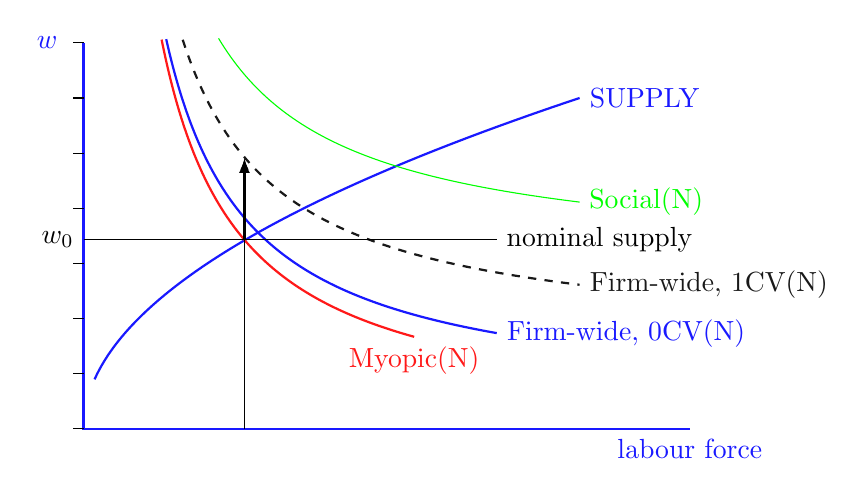
\begin{tikzpicture}[scale=.7]
%\def\bndmax{5}        %https://tex.stackexchange.com/questions/68462/filling-a-complex-region-with-tikz
%\def\bndmin{0.2}
\def \Y {7}  % height of y axis pecent
\def \W {15}  % length  of x axis
\def \Wbar {3} % jmeam wealth
\def \omega {3}
\def \A {1}  %was .5
\def \B {.5}

\draw [thick, color=blue!90] (0,\Y)node[left=.2cm]{$w$} -- (0,0)--(\W-4,0)node[below]{labour force};  
 \foreach \yi in {0,...,\Y} \draw (0,\yi)--(-.2,\yi)node[left]{};
 
\tikzset{func/.style={thick,  color=blue!90}}
\draw[ func, domain=.2:\W-6] plot [samples=200] (\x, 2*\x^.5)node[below=.1, right]{SUPPLY};

\tikzset{func/.style={  color=green}}	
\draw[func, domain=2.45:\W-6] plot [samples=200] (\x, 10/\x+3)node[above=.1, right]{Social(N)};

\tikzset{func/.style={thick, dashed, color=black!90}}	
\draw[func,domain=1.8:\W-6] plot [samples=200] (\x, 10/\x+1.5)node[ right]{Firm-wide, 1CV(N)};

\tikzset{func/.style={thick, color=blue!90}}	
\draw[func,domain=1.5:\W-7.5] plot [samples=200] (\x, 10/\x+.4)node[below=.05, right]{Firm-wide, 0CV(N)};

\tikzset{func/.style={thick,color=red!90}}	
\draw[func,domain=8.5/6:\W-9] plot [samples=200] (\x, 10/\x)node[below]{Myopic(N)};

\draw(0,3.425)node[left]{$w_0$}--(7.5,3.425)node[right]{nominal supply };
\draw[thin,-latex](2.92,0)--(2.92,4.9); %a vertical labour supply
\draw[thick,-latex](2.92,3.425)--(2.92,4.9);
%\draw [blue,  thick](13, 8.3)--(15,8.3)node [right, black] {\small A=\ 1,\ B=0.5};
%\draw [green, thick](13, 7.6)--(15,7.6)node [right, black] {\small A=.8, B=0.8};

%\node at (5,-1.5){Resulting in  profits, expansion, and/or entry: the city grows};
 \end{tikzpicture}
\caption{Multiple marginal products}
\label{fig-growth-amenity.tex}
\end{center}
\end{figure}

 Figure~\ref{fig-growth-amenity.tex} illustrates the labour supply curve and the four versions of MPL that arise for any standard production function with diminishing marginal product of labour and agglomeration effects of the sort we model. These agglomeration effects account for O'Sullivans axioms (b), (c) and (d) for this and similar models. 

 
\subsubsection{Output and wage}
We need a combination of classical and neoclassical distribution theory.

City output is divided among the classes of society. Neoclassical theory suggests wages are allocated according to marginal product and classical theory suggests rents according to the pattern of ownership.

Equation one, in effect determines a wage, (Given the observed values for the scaling coefficients for total wages and labour, $bW < 1.15$ and $bL < 1$, )  although there are many possible distributional specifications and many possible labour market and firm structures. Bettencourt provides two  estimates,  1.11 and 1.35, for the scale factor for urban personal income in the Brazil and South Africa respectively. A more recent  study supports the Bettancourt results for China.\footnote{Wu W, Zhao H, Tan Q, Gao P. An Urban Scaling Estimation Method in a Heterogeneity Variance Perspective. Entropy (Basel). 2019 Mar 28;21(4):337. doi: 10.3390/e21040337. PMID: 33267051; PMCID: PMC7514821.} 

\subsubsection{Wage and city size}
The third determines the extent of the city. This comes form the Alonso model discussed in chapter XXXXA. 

% PROBABLY REMOVE - FIGURE REPEATS
\begin{figure}
    \begin{center}
     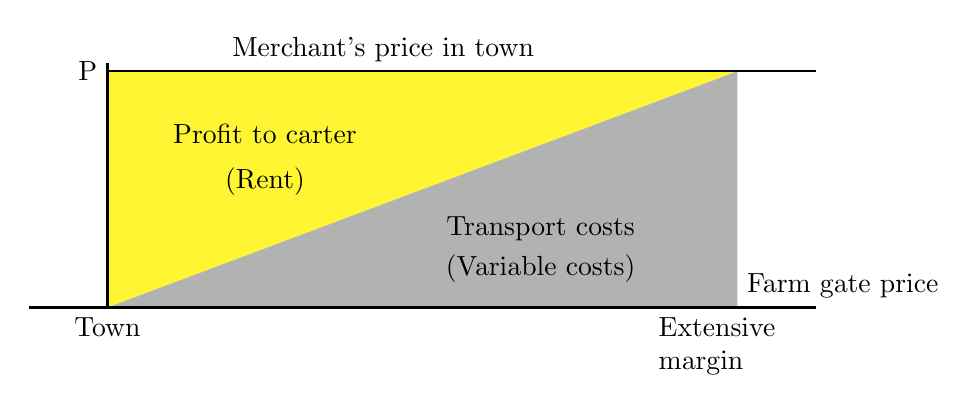
\begin{tikzpicture}[domain=0:2]
%\draw[thick,color=gray,step=.5cm, dashed] (-0.5,-.5) grid (3,3);
%\draw[line width=.01, green ] (0,0) -- (10,0) node[right  ] {Distance};
\node at (1,0) [below] {Town};
\fill[yellow!80]  (1,0) --(9,3)--(1,3) --cycle;
\fill[gray!60] (9,3) --(1,0)--(9,0) --cycle;

\draw[thick ] (1,3)node[left]{P}  -- (10,3);\node at (4.5,3)[above ] {Merchant's price in town} ;
\draw[thick ] (0,0)  -- (10,0); 

%\draw[thick,color=red] (1.5,0) -- (1.5,1) node[below right] {Fixed cost} -- (1.5,1.5) --(10,3.25)node[above left] {total cost};
\draw[thick] (1,0) -- (1,3.1) ;
\node[below,text width=2cm]at (9,0) {Extensive margin};
%\draw[ultra thick, blue,<-> ] (3,1.8) -- (3,2.5)node[left] {annual rent at a} -- (3,3) ; 
\node at (9,0)[above right] {Farm gate price};
\node  at (6.5,1){ Transport costs};
\node  at (6.5,.5){ (Variable costs)};
\node  at (3.,2.2){ Profit to carter};
\node  at (3.,1.6){ (Rent)};
\end{tikzpicture} 
    \caption{Transport costs, the yellow area, take a share of the profit for vegetables sold in the town}
    % \label{fig-rent-ricardo}
    \end{center}
\end{figure}

\begin{figure}
    \begin{center}
    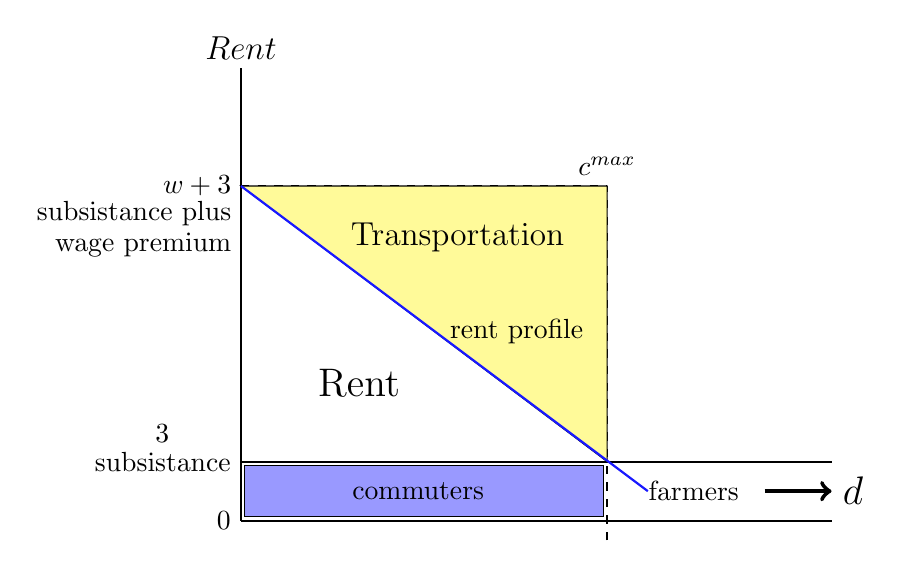
\begin{tikzpicture}[scale=.5]
\def\bndmax{5}        
\def\bndmin{0.2}
\def \n {10}  % height of y axis
\def \d {15}  % length  of x axis
\def \t {.75}  %  cost of transportation per unit x
\def \th {1}   %
\def \w {7}    %  wage premium
\def \om{1.5}%  omega =rural wage Zero for urban population
\def \azero{2}
\def \aprime {-.0}	
\tikzset{func/.style={thick,color=blue!90}}	
\draw [thick] (0,-\om) --(\d,-\om);  			% Zero for rural population
\draw [thick] (0,-\om)node[left]{$0$} --(0,\n);	% Y axis
\node at (0,\n+0.5){\large$Rent$};

\draw [thick] (0,0)node[left]{subsistance}--(\d,0);
\node a t(-2,.7) {$\omega$};
\node[left] at (0,\w){$w+\omega$};
\node[left] at (0,\w-.7){subsistance plus};
\node[left] at (0,\w-1.5){wage premium};	
\draw [dashed, thick](9.3,-2)-- (9.3,\w)node[above]{$c^{max}$};
\draw [dashed, thick](0,\w)-- (9.3,\w);
% solid color for commuters
\draw[fill=blue!40] (0.1,-0.1) rectangle (9.2,-\om+.1);
\draw[fill=yellow!40] (9.30,7.) -- (0,7)--(9.30,0.)--cycle;% Rent \w-.2
\draw[func,domain=0:\w/\t+1] plot [samples=200] (\x,{\w-\t*\x});
\node at (5.5,5.7){\large Transportation};
\node at (7,3.3){rent profile};		%Rent Profile	
\node at (3.,2){\Large Rent}; 		%Rent 
\node at (4.5,-\om/2){commuters};
\node at (11.5,-\om/2){farmers};
\draw [ ultra thick, ->](13.3,-\om/2)--(15, -\om/2)node [right] {\Large $d$};
\end{tikzpicture}
    \caption{A circular city with uniform transportation costs.}
    \label{fig-rent-alonso}
    \end{center}
\end{figure}

A simple case is the circular city with uniform transportation cost, $t$. \[r^*= \frac{w}{t}\]% A more complex model might have density depend on location, for example, in the continous circular cityt\,
If transportation costs vary by  distance we might have something like this constraint on extent\[w=\int_0^{d*} t(d)dt.\]

This approach imposes an equilibrium condition on the model. It is unnecessary working with a citation of known extent and density. The analytic approach is easily extended to variable transportation cost, although at the expense of additional computational complexity.

\subsubsection{City extent and population}
Equation  four  closes the model by linking the extent of the city to the population. A simple case is the circular city with uniform population $d$, where $d$ is density per unit area and $r^*$ is the radius of the city: \[P=d\pi r^{*2}\] 
More generally, density might vary with for example, the distance $r$ from the centre of the city:
\[P=\pi \int_{0}^{r*}d(r)\,dr\] 
In a computational model a table of densities would provide the link.



\subsubsection{challenges}
maybe discuss some of the modeling challenges - division of income, lags, ???

\vspace{2cm}


\subsection{Cities becoming productive}
 The growth of many cities was initially fueled by agricultural rents and resource exports. The industrial revolutions transformed many of these consumption cities into thriving production centers. 

while the ``origins'' of consumption cities can be traced to (i)
resource rents, (ii) rents from agricultural exports in countries with sufficiently high agricultural productivity, and (iii) ``premature'' deindustrialization.  Source:
%\href{https://www.brookings.edu/blog/future-development/2022/07/14/1622441/}
{Are cities engines of production or consumption, and does it matter?}


\section{Model assumptions}
\begin{enumerate}
\item There is full employment, no frictional unemployment, and no labour adjustment costs.
\item Firms set output and factor inputs to maximize profits, so factors are paid the value of their marginal private product
\item Demand for output is perfectly elastic (constant price = 1)
\end{enumerate}


Rural producers pay a wage $\psi$. this covers a standard house, lot, entertainment, diet and consumption pattern. We  choose units so that per-period cost of a unit of productive capital is also $\psi$





\chapter{Model}



\section{OLD Implementation}


Household agents have:
\begin{enumerate}
   \item A home. Agents live somewhere, inside or outside the city,
   \item finances: they have assets, a housing budget, income, and a spending pattern - family lending pattern  
   shaped by profession, demographics, family structure, etc.) - risk profile
   \item utility function: they have a utility function with location  preferences - amenity, open space, house size requirements, transportation costs - shaped by profession, demographics, family structure, etc
\end{enumerate}	

Buyers then consult with a financial agent to determine the maximum mortgage and interest rate they'd qualify for based on their income. This gives an upper bound to the range of homes they may consider. 

Finally agents valuate the homes offered and place bids. % For simplicity of implementation, they place bids on all homes they consider. 

%Calculate willingness to pay
%Consider options
%Place bids
%
%Calculate willingness to pay (urgency/position on the market)
%Assess need for housing
%- Urgency of need Unhoused, sold house or served notice? 
%- Family or demographic changes
%- Financial viability of current situation
%Assess financial situation
%Get Max mortgage and max carrying cost given income and wealth from a bank
%Get options from real estate agent
%Place bids based on xy
%Consider options
%Place bids
%
%BUYER
%Enter market to buy
%Decide level of urgency (or decide with prospect theory - functional form for optimism/urgency/time to choose)
%(income/wealth)
%Maximum mortgage 
%Maximum carrying cost
%Household attributes - household size, employment location, amenity
%Current housing
%
%Realtor gives list of houses to look (real estate search -e.g. price range)
%Place offers - low if can't afford, higher if market is tight
%If failed, consider renting or buying next time.

\begin{figure}[htb]
    \begin{center}
 \tikzstyle{decision} = [diamond, draw, fill=blue!20, 
     text width=4.5em, text badly centered, node distance=3cm, inner sep=0pt]
 \tikzstyle{block} = [rectangle, draw, fill=blue!20, 
     text width=5em, text centered, rounded corners, minimum height=4em]
 \tikzstyle{line} = [draw, -latex']
 \tikzstyle{cloud} = [draw, ellipse,fill=red!20, node distance=3cm,
     minimum height=2em]
%
 \begin{center}
 \begin{tikzpicture}[node distance = 2cm, auto]
     % Place nodes
     \node [block] (need) {Assess need for housing};
     \node [block, below of=need] (finance) {Assess financial situation};
     \node [block, below of=finance] (alternatives) {Select homes to consider};    
     \node [block, below of=alternatives] (bid) {Place bids on homes};    
     % Draw edges
     \path [line] (need) -- (finance);
     \path [line] (finance) -- (alternatives);
     \path [line] (alternatives) -- (bid);        
 \end{tikzpicture}   
 \end{center}
    \caption{Worker housing flow chart.}
    \label{fig-code-worker-choice}
    \end{center}
\end{figure}

\subsection{Initial conditions}
Initialize the model with grid. Each element contains 1 housing unit.

The model space is divided into a uniform grid of single family homes % Additions: apartment buildings, a mechanism to subdivide homes, rent bedrooms, accumulate adjacent land and build new higher density buildings, an urban land boundary, a mechanism for wealth agglomeration through density.

The social structure of the model begins with urban workers who commute and earn wages in the urban commuter-shed, and rural residents and landowners who may choose to move to the city. 
We imagine the initial set of workers in our city commuting daily, being paid monthly and residing in urban housing for their working lives, which are arbitrarily set. 

Initially all urban workers are also homeowners. When we allow the initial urban residents to retire, they may sell or rent out their properties to new workers. This introduces an additional \gls{class} of resident, the urban tenant. The final agent in the model is a `bank' that represents both the financial sector and the owners of financial capital. The bank provides mortgage funds can %may actively 
purchase land as a financial asset on behalf of investors.

\subsection{Model Steps - Housing market}
% Figure xyz traces the flow. 
In each time step agents firms update wages and job availability, agents decide whether to work and whether to buy and sell homes.
 % Schedule: Multi step by breed
 % Steps Labour
 % step - workers: market/production, enter market to buy, list properties real estate agent matches agents - has bids 
 % bidding - workers and firm consider properties and make bids (2nd step or spread over 2 steps)
 % negotiation - sellers consider and accept bids (or real estate agents manage negotiation)
%Buyers evaluate their need for housing.
% Agents decide whether to enter the housing market as a renter or a buyer.

at every time step 
    1) Some new tenants arrive into the city
    
    2) All unhoused tenants look for a housing unit 
    
        a) They have to decide whether to buy or rent. Decision depends on their income, and the availability of Corporation of Public Housing loans 


        b) If they buy, they seek apartment and evaluate, and place a bid (see ALMA)
        
        c) if they rent, they look for an apartment that matches xyz criteria, and place request to rent. Rental is given by the landlord to the first tenant that matches the asking rental price. 


Workers give up their search and leave the city if they do not find a housing unit 

%\chapter{Background Rought Notes - Rent History Etc}



\section{Agglomeration discussion}

The phenomenon of growing productivity was initially identified and estimated in the economics literature production at the national level. The estimated functions linked capital and labour inputs to output.  Soon after the  earliest econometric models of output  were estimated, it was found that equations were not stable over time. Productivity grew over time
(We can do the arithmetic with the cobb douglas to illustrate) 

Faced with this puzzle, Robert Solow introduced a term that was time dependent, and an entire literature developed to explain this term. One productive stream explained growing productivity in terms of agglomeration effects- more people, more workers more firm or more diversity of firms appeared to be associated with growing productivity. Two major schools emerge - roughly speaking,  the Marshallian explanation, which emphasized firm-level processes and the Jacobs model which focuses on the creative effect of agglomerations of people in cities. Both have receives empirical support.

(We can do the arithmetic with the Cobb Douglas to illustrate)

Louis M. A Bettancourt and others applied similar models at the level of cities, but rather than a time-dependent term, they introduced a population-dependent term and found evidence from cities around the world that productivity rose as population rose: The scale of the city has a positive effect. The result  was one of a wide range of scaling results identifies in a great variety of systems examined in the complexity literature 


\section{Background}

\subsection{Inequality}
this wasn't how capitalism was supposed to work
wages part, 
over 50 for rent

\subsection{Drivers of the housing crisis}
supply and demand, stagnant income, and finacialization of housing

Several explanations of the current situation are commonly proposed. The first is simply that the problem of housing is a supply and demand problem where supply is blocked by some features of urban regulation. The second explanation is that the distribution of income has changed in some way that mean a significant fraction of the population are unable to afford satisfactory housing, and therefore this is the problem that must be solved.  The third common explanation currently is that financialization of the housing market  is changing the way the city economy is working, redistributing income and potentially threatening the long term growth and wealth creating capacity of the city.


\subsection{How we do the resilience analysis}

- what will we do? *** 



\section{Rent, Production and the City: Who Gets the Wealth}


%The sources of economic growth and the distribution of income are themes that run through the history of economic thought. 

The story of rent is the story of 

two great theories of distribution
a methodological evolution from descriiption to calculus to complex systems and an evolution of the economy 
from agriculture to indsutrial produciton, to social scaling or wealht in cities. 



There are two great stories of distribution in economics. The first and oldest is rent, %the classical work on rent, going back to 
developed in Ricardo, in which owners of an asset are able to extract a value beyond what they contribute. 
The second is the marginalist approach, developed by Clark and others, looking at a scenario in which workers receive the marginal value of their contribution to production. This tradition dominate in neo-classical economics, particularly in the United States, and %formed the basis of conventional micro-economics training.
% it gave a story of production that seemed to align with the rising fortunes of ordinary people/workers following WWII, in the 1950s and 1960s when it came to dominate. 
% formed an intelectual foundation for anti-monopoly political movements in the early 20th century. 
This work contributes to a third theory of 

emergent complex systems methodology and  work on urban science, the power law concentration, and integrates/ to achieve a sysnthesis of  the clasical descriptive work on rent and the neoclassical marginalist appraoch

These stories are, at their heart, stories of who claims what share of production. They evolved within an evolving theory of production. The early stories of production thinkers like Ricardo focuses on were agricultural. Who claimed the surplus from agricultural production? Over time, the story moved to industrial production, and increasingly urban- with the social wealth of cities/human capacities developed in cities dominating. % Later thinkers including Smith and Marx%leaving aside purely inherited weath- as that becaumse caught in this same circuit of capital transforming from production, to money and back. 



Methodological-- early discririptive theories told rich layered stories with different
The excitiment concentrated  calculus.. in the classical distributional dynamic.

The complexity - allows for tracing the paths of individual- what happens for whom under a far broader range of conditions

The clarity of pedagogical methcs- bottom up and top up both have illustrative cases e.g. edgeworth box or the schellings/birds models.
But true theory integrates in something that moves between scales fluidly, makes itpossible for the distinct scale based approaches to come together.


Complexity

Early discriptive work
This explosion of formal rigour - focused attention.. 


And the political context..

Monopoly- political pressure real explosion ofwealth creation-- economic success of political efforts to break up monopolies.
And a dynamic- lots of worker power- expanded equality-- workers seemed strong, 
As well as the political environment in the US during the cold war, older stories rooted- marx- repression, ednomists perhaps created an envronment in which economists
a side fo the economcs

-- methological pdrived moved the point whre discriptive and historical appraoches baredly taguth.

Samuelson-- successful exciting-- formal-
a generation
created micro, macro
-- at the moment of the baby boom- departments founded in this moment of exuberance. raised in it, taught according to this framework.


Computers took over from calculus -Brian Arthur
Cities took over from industries - concentrated value-- finance- and law main power centers.. - eigen value centrality.

Crisis in 2008 -- reintroduced dscrptive
Methodologial
Cities-- power law dist. rising debt and inequality. -- unstable and financialize.d
Increasing inequality, risind debt. - worker power expanding wages and equality, a story that explained- vs subsistence.


Exactly what those pattnersnew methods are so succesful are what was lef tout..



Polarized in the periodo of the cold war - the discussion of the market-- perhaps a tendency to avoid the distributionl.. Revolution and drama.



Early theories were implicit. They have the same logic- but exist in words

mathematization was important to the simple centrality of marginalism.






With Clark
A second great theory of distribution
The result is much of the theory of rent was lost. 
time

While Marx emphasized the tendency towards consolidation and exploitation in markets, Clark saw the tendancy to increased competition. 

This allocation— dynamic quality of how wages evolved
They are bidding- and it will converge 
What share do workers get- subsistence wages- get 
But as output grows, and as firms compete for labour, particularly skilled labour, is that a sufficient experience.



Three drivers
Calculus had limits.
The political moment of expanding wages with a labour sector in a position to negotiate as the economy rebuilt following WWII and destruction of old wealth— dynamic time. 
Following WWII with growing demand for labour labour could bargain, 
Following WWII in the period— subsistence waves tending— when labour could bargain,
Following break up some of the largest monopolies like in steak— general steal


Also coincided with the political movement McCarthiesm perhaps led scholars to de-emphasize the connections of their work with the classical socialist litturatue.
Mathematical economics became an exciting and dynamic area.

Until this point the theory was largely descriptive..
xx Cobb working with Douglass developed a formulation — exponential, in economics their names have remained associated with the xyz formulation. 

Clark made a case it was just- became problematic.
Doesn't actually happen -- and not jsut

OUR CASE IS THAT IT FALLS OFF A TOTALY DIFFERENT CLIFF



Economics had theories with rich dynamics, concerned 
Classical economics was concerted with ownership and wealth. But they were largely descriptive.
But the new calculus struggled to deal with stocks and with dynamics. 
(Came back with forester and other systems theory, as well as complexity etc.)

The French Engineers in the school of bridge end road used calculus early .. followed by xyz
Technical development and intelleual excitement aligned
Became very exciting dynamic, had many success - took over the discipline. 
Tied with political successes breaking up big monopolies — seemed to offer a path forward

US opposed soviet ideas and an intellectual environment that may have led academics to dephasize the aspects of their thinking connected with classical socialists thought. 

In this environment a particular approach became dominat— also at a moment when schools and departments were growing— the baby boom came to universities at the moment of Samuelson’s peace micro-macro divide gave a tool kit to a whole generation of economists— 

Embedded at the heart of micro- the satisfyingly precise formal structure of calculus.. the marginalize appraoche— 
Thus came to define a new disciplien— a formalization of Econ.. 
Extensions from that base became the defining advances of a generation of American economists..
Attracted math- a feedback loop.

Less emphasis on intellectual history, how changing- heterodox.. all the full range of thought

Including the much more exiting new techniques of complexity and systems- opening in 2007 an explosion of these techniques in the economies. 




CITIES

But cities matter more and more
Jacobs theory of wealth and value as fundamentally social.. 
Combined with xysz. Jacobs did

Now complexity and scaling theory revealing the universality of those principles advanced by Jacobs..

This requires a different formulation of rent… - and production wealth is inherently social what are the implicaitons— what does that mean.. 






In our model, land comes in implicitly through the demand for labour. 


\section{Chapter: Draft Literature Review and Background}

\section{Background}
\label{Sec:Background}
\newpage
Our approach/model is constructed, drawing together pieces from a number of research areas from economics and the study of cities, including rent theory, production functions, the standard urban model, growth theory, urban growth theories, financialization and the theory of distribution. 
We relate this to the scaling models from the study of complexity. This gives a deeper look at distribution in the cities, the effect of financialization, and effect of both of these on the growth and development of cities. 

The literature makes it clear that the cost of transportation is crucial, the cost of housing is crucial, and that there are strong pervasive agglomeration effects driving productivity and population growth. (City population is observed to follow a power law distribution.)

We are interested in agglomeration economies. The wage  structure would then be related to the population or industry  structure. Externalities driving agglomeration may be classified  into two types, the  or so-called ``Marshalian''  and ``Jacobs'' externalities


3 lines  
- production leading to Jane Jacobs
- cities leading to Jane Jacobs
- scaling factors and complexity leading to Jane Jacobs and empirics in a theory of cities

2 theories of production

Ricardo
Ricardo’s rent theory explained class and the distribution of income in terms of the the productivity and ownership of land in an agricultural society. Land was the scarce factor in production and control of land allowed landowners to extract any production in excess of the agricultural wage. Ricardo could assume that labour was in surplus and therefore the agricultural wage would approximate the subsistence wage. 

Marx
Marx adapted the Ricardian model to an industrial society in which surplus product could be used to create more capital and largely ignored land rents. He retained the subsistence wage, and explored the effect of reproducible capital.

Clark
Clark %\footnote{and Wicksteed} extended the theory of rents to produce 
elaborated a neoclassical distribution theory that tied income to the marginal product of each factor for a firm in a competitive economy rather than class ownership of capital. 
This marginal productivity theory became dominant SOME BENEFITS.. Although the marginal productivity theory became dominant in economic thinking, rent theory retained an important explanatory role in resource, agricultural, regional and later urban economics and even sports economics. 

Clark %\footnote{and Wicksteed} %extended the theory of rents to produce 
elaborated a neoclassical distribution theory that tied income to the marginal product of each factor for a firm in a competitive economy rather than class ownership of capital. Although the marginal productivity theory became dominant in economic thinking, rent theory retained an important explanatory role in resource, agricultural, regional and later urban economics and even sports economics. 

Rent theories have remained at the centre of economics despite the development by Clark (1894) of the more modern theory of distribution in which factors ideally receive the value of their marginal product. In modern welfare economics a measure of surplus that is the direct descendent of Ricardian land rent is at the core of the First Theorem of Welfare Economics, arguably the most significant theorem in the social sciences. With Alonso (1964), another another application of rent theory became the foundation of modern urban economics.

\section{Exploitation}
John Roemer’s 1982 Class Exploitation Correspondence Principle (CECP) states that producers who optimize by only selling labour are exploited at the economy’s equilibrium, and agents who optimize by hiring labour are exploiters. Exploitation and class structure are shown to arise from differential endowments in a manner consistent with both Ricardian explanation of class incomes and Marx’s conception of exploitation. We extend the argument to show that differential access to finance capital, urbanization, the growing importance of human capital in producing surplus and agglomeration economies endogenously generate a class structure based on the indirect capture of land rents, We illustrate the emergence of class structure within a simple agent-based model of the land market in a monocentric city. The model is consistent with the theories of Ricardo and Henry George in locating the ground of exploitation and class in the capacity to extract social surplus through land ownership, and differs from the standard Marxian analysis in its reliance on access to financial capital rather than control of productive physical capital.

The sources of economic growth and the distribution of income are themes that run through the history of economic thought. 

From Smith and Ricardo economist have understood that the net product of the economy is divided among functional classes.
 Ricardo is generally credited with providing the best early description for the division of the product of the land between labour and property owners. 
 Marx is generally credited with providing a convincing explanation based essentially on Ricardo's insights, of the distribution of the product of industrial capital with a class-monopoly on ownership the capital,  as well as insights about the evolution of a society based increasingly on produced rather than natural capital. 
 Henry George elucidated the role of land rent, particularly in the urban context as as a mechanism for extracting socially produced economic surplus.  

The division of the product of the earth among the classes of society has been a central issue in economics since at least Ricardo presented his theory of  rent, through Marx, adapted the concept of rent to an industrial and capitalist economy and Henry George, who applied it in the urban context. Land rent is also at the core of modern urban models.  John %\textcite{RoemerGT} 
in \textit{A General Theory of Exploitation and Class} 

%\textcite{RoemerGT} 
%\footnote{\cite{RoemerGT} p12} 

The distribution of rent, where it goes, and what the implications are. 

\section{Liturature Review}

3 lines  
- production leading to Jane Jacobs
- cities leading to Jane Jacobs
- scaling factors and complexity leading to Jane Jacobs and empirics in a theory of cities

2 distributional stories.
- class and rent -- synthesis of rent and class--

Then is the history of rent seperate?

O’Sullivan (2011) identified “five axioms of urban economics” that have emerged from a century of study: (a) location-specific costs and benefits balance to generate a locational equilibrium; (b) self-reinforcing effects induce concentration of activities and individuals; (c) externalities are prevalent; (d) production is subject to economies of scale, which favours agglomeration; and (e) competition generates zero economic profit. These features combine to produce dynamic urban system that will shape our future. 

We build a model that incorporates the five “axioms” to demonstrate how production externalities, in a class of models, can drive urbanization, class formation and the wealth distribution.

To understand the relationship requires integrating the distributional appraoch from clasical economic theory of rent with the modern marginalist model of distribution through wages. It does this by integrating the urban model with the model of production and including the cost of land and transportation in the urban wage in the labour costs. 
In this way the two factor model of projection reflects the clasical landowning extraction of rents by landowners, with a model of wages in competitive markets. 

\subsection{Rent}

 What Is Economic Rent?






neoclassical story.
Economic rent is an amount of money earned that exceeds that which is economically or socially necessary. This can occur, for example, when a buyer working to attain a good or service that is considered exclusive makes an offer prior to hearing what a seller considers an acceptable price. Market imperfections thus lead to the rise of economic rent; it would not exist if markets were perfect, since competitive pressures would drive down prices. 
%https://www.investopedia.com/terms/e/economicrent.asp
% https://www.wallstreetmojo.com/economic-rent/



Henry George brought the classical position to its logical conclusion: rent is an unearned increment. The Classical Base of Modern Rent Theory, Conway L. Lackman
“Whatever part of the produce or… of its price, is over and above this shame” (which pays for the capital advanced “together with the ordinary profits”), “he” (the landlord) “naturally endeavours to reserve to himself as the rent of his land” ([O.U.P., Vol. I, p. 163; Garnier,]  
l.c., p. 300). Theories of Surplus Value, Marx 1861. [Chapter XIV]  
 Adam Smith’s Theory of Rent [1.  Contradictions in Smith’s Formulation of the Problem of Rent]
This excess may “he considered as the natural rent of land” ([O.U.P., Vol. I, p. 163; Garnier,]
l.c., p. 300).


 \subsection{Ricardo}
 
 David Ricardo developed a theory of land rent.
Leading figure in classical economics



He modelled the agricultural economy.
Ricardo developed the idea of 

He was friends with James Mill, Jeremy Bentham and Thomas Malthus.

He theoriezed the agricultural economy.





\section{Drafting REVIEW}
This section traces the history of rent and production in economics.
 central issue in economics since at least Ricardo presented his theory of  rent, through Marx, adapted the concept of rent to an industrial and capitalist economy and Henry George, who applied it in the urban context. Land rent is also at the core of modern urban models.  


In economics, rent is a surplus value, i.e. the difference between the price at which an output from a resource can be sold and its respective extraction and production costs, including normal return (DFID, 2003; Luchsinger \& M\:uller, 2003; Sharp, 2003; Stoneham et al., 2005).

Chapter 24: Doctrine of Adam Smith concerning the Rent of Land
``Such parts only of the produce of land,” says Adam Smith, ``can commonly be brought to market, of which the ordinary price is sufficient to replace the stock which must be employed in bringing them thither, together with its ordinary profits. If the ordinary price is more than this, the surplus part of it will naturally go to the rent of land.

If it is not more, though the commodity can be brought to market, it can afford no rent to the landlord. Whether the price is, or is not more, depends upon the demand.''

More briefly, rent is a surplus value after all costs and normal returns have been accounted for. Normal costs include  payment of all the factors of production at their market rate.(Labour at the going wage, Capital at the interest rate, supplies at their normal price). The great social question at first was who gets the surplus.  

%The question was pressing because it appeared that landlords were capturing the surplus without contributing to production while may peasants were very poor. 

Ricardo

% Born in the late 1700s, was a British poltical economist. The son of a stockbroker, he built a fortune by investing.
The law of rent was formulated by David Ricardo around 1809, and presented in its most developed form in his magnum opus, On the Principles of Political Economy and Taxation. This is the origin of the term Ricardian rent. Ricardo's formulation of the law was the first clear exposition of the source and magnitude of rent, and is among the most important and firmly established principles of economics.

The landlord would rent out all the land which generated at least enough to pay all the costs. Anything in excess of the costs could be charged as land rent to a tenant farmer.

This excess, or surplus, he identified as the income of the landlord. The landlord captures the surplus by ownership of the natural resource land. 

Ricardo, did not write down a production function his, but his analysis can be understood as implying one.

Clearly in his model there are two basic productive factors, land and labour. The landlord  receives the surplus generated by the land and the rest of the value of production goes to labour. Ricardo essentially assumes that there wage is  just sufficient to reproduce the labouring class.\footnote{``In the natural advance of society, the wages of labour will have a tendency to fall, as far as they are regulated by supply and demand; for the supply of labourers will continue to increase at the same rate, while the demand for them will increase at a slower rate.''  This is  basically Malthus.} He has explained the distribution of the fruits of the land among the main classes of the economy.

The implicit production function is
\[Y=F(N, L)\]

Where the output $Y$ is a function of $N$, the number of workers and $L$, land.

His analysis included a concept of diminishing marginal return, the rate at which production grows declines. 
This shows in his use of the terms ``extensive margin'' and ``intensive margin'' to explain the income of the landowner. He focused on the difference between the cost of production on a unit of land and the revenue generated. 



employers enjoy a bargaining advantage over workers and can coerce them to accept worse terms, because they need individual workers less than individual workers need employment. It is no surprise Marx was an admirer. Wages are not the simple product of supply and demand in Smith; bargaining asymmetries are key.

Ricardo included concept of diminishing marginal product, which means


His analysis can be understood in terms of a production function. 
% Factors of production are things that play a role in creating the output. There are several factors of production, things required for production/to create wealth/value (using capital and labour). Most obviously capital and labour. One of the factors of production is labour. In principle the rate at which hiring changes output can take any form. If hiring one more worker increases output, the marginal product of labour is positive. The marginal product can be positive and increasing, or positive and decreasing. If the marginal product of labour is decreasing, the curve is slopes downward, there are decreasing returns to scale, and each additional worker adds less to output than the last. % DIAGRAM  In general hiring more people increases production. In general employers choose workers who would increase production. Otherwise they would not hire. Returns to scale determins how much hiring one more worker increases output. With increasing returns to scale, each new worker increases output more than the last one did, and companies tend to grow big. With decreasing returns to scale, each new worker increases output by less than the last one did and so more, smaller companies may form % (TODO: clarify explanation of implications). To connect with the tradition of analytic economic modelling, ensure there is an equilibrium, by making the marginal product of labour monotonically declining, ors declining over the whole function. This equilibrium condition ensures the curve in the diagram is slopped downward and the curves intersect. % (TODO: discuss/justify assumption, ground empirically)


 2 factors is typical since it's enough for most kinds of analysis. Another factor typically used to introduce another constraint on production, or potentially consumption. Eg. labour is mobile, capital takes time to accumulate but you can put it anywhere, but forest is a flow from the ground-- puts a limit on the region of the city. - land, flow from the land, natural resources.
 
 The factors are usually chosen so xyz
 To keep it tractable- one which is slow to adjust and one which we can adjust quickly - one which is world/embodied work and one which is current work, the rest falls between.

%and is replaced with capital. -- What you'd do an analysis if you put in 30 factors, in the analysis you hold 28 and let 2 move to see what's going on, and what you get is - you have a production function with certain mathematical factors, you can expand as much as you want. you can expand as much as you like-- everything you deduce about 1 is true about any 1 and all the rest if they hold the same functional relation to one another.This is a mathematical trick that gives you xyz.. things you get from it are things like there's a good reason to assume growth till you get 0 profit, then you get competitive markets, all that drops out of the math. - profit maximization you can impose, expansion to 0 profit, expansion till marginal product of labour equals the wage, value of marginal product of capital equals the interest rate, marginal product of whatever is equal to the price/unit of whatever it is - 


Historic evolution is land and labour.

Marx


, as we move from agriculture, 





John Roemer’s 1982 Class Exploitation Correspondence Principle (CECP) states that producers who optimize by only selling labour are exploited at the economy’s equilibrium, and agents who optimize by hiring labour are exploiters.

Roemer
RoemerGT demonstrates that in equilibrium there are classes that are exploited and classes that are exploiters, as well as intermediate cases, using  a definition a definition of exploitation 

that is essentially Marxian and is consistent with Ricardo's rent theory and that of Henry George: 
%\begin{quotation}
%
An agent is exploited  if and only if the value of the labour the agent sells plus the value of own production plus wage earnings is less than the maximum value of their consumption bundle.
%\vspace{.25cm}
%
%and\vspace{.25cm}
%
%An agent is an exploiter  if and only if the value of the labour the agent sells plus the value of own production is less than the minimum value of their consumption bundle.
%\end{quotation}

A General Theory of Exploitation and Class examined a General equilibrium linear economy in which all individuals rationally choose their  activities given their initial endowments and demonstrated  the endogenous emergence of a class structure in a purely neoclassical model. 

Marx
distribution of the product of industrial capital with a class-monopoly on ownership the capital,  as well as insights about the evolution of a society based increasingly on produced rather than natural capital. 



CITY
Rent howerer has remained central in the study of the city
Began everywhere.

Johann Heinrich von Th\"unen was influential in developing the spatial analysis of rents, which highlighted the importance of centrality and transport. Simply put, it was density of population, increasing the profitability of commerce and providing for the division and specialization of labor, that commanded higher municipal rents. These high rents determined that land in a central city would not be allocated to farming but be allocated instead to more profitable residential or commercial uses. 


 Henry George elucidated the role of land rent, particularly in the urban context as as a mechanism for extracting socially produced economic surplus.  

OLD?
 
Ricardo developed a theory of land rent. He did not write down a production function, but he quite clearly understood and used the concept of diminishing marginal product. This shows in his use fo the terms ``extensive margin'' and ``intensive margin'' to explain the income of the landowner. He focussed on the difference between the cost of production on a unit of land and the revenue generated. The landlord would rent out all the land which generated at least enough to pay all the costs. Anything in excess of the costs could be charged as land rent to a tenant farmer.

This excess, or surplus, he identified as the income of the landlord. The landlord captures the surplus by ownership of the natural resource land. 

Clearly in his model there are two basic productive factors, land and labour. The landlord  receives the surplus generated by the land and the rest of the value of production goes to labour. Ricardo essentially assumes that there wage is  just sufficient to reproduce the labouring class.\footnote{ ``In the natural advance of society, the wages of labour will have a tendency to fall, as far as they are regulated by supply and demand; for the supply of labourers will continue to increase at the same rate, while the demand for them will increase at a slower rate.''  This is  basically Malthus.} He has explained the distribution of the fruits of the land among the main classes of the economy.

The implicit production function is

\[Y=F(N, L)\]

Where $N$ is the number of workerrs

\subsection{Marx}
 Marx examined a developing manufacturing economy. In this economy the owners contributed the machinery, buildings, and even working capita to fund the workers until the product can be sold. This contribution must be accumulated from their profits in the preceding cycle of production,  and has to be reinvested once the revenues of the current round have come in and the bills have been paid. Marx actually describes a circuit of capital from its for as money to its form as physical capital. 
 
 
The implicit production function is

\[Y=F(N, K)\]
where $K$ stands for the productive capital stock. 

As in Ricardo, labour is in surplus and capital is scarce. As in Ricardo the scarce factor owned by a special class - now the capitalists, is able to appropriate the is able to capture the surplus value. Like Ricardo,  marx saw the appropriation of surplus as without morel justification - 


Marx also pointed to a new dynamic in capitalist systems - that productive capital is not fixed as land is, but does and must expand as surplus is reinvested. The expansion will eventually outrun the expansion of demand and the rate of return will fall, leading capitalists unwilling to invest and creating a crisis,.


 
\subsection{Henry George} 
  Henry George returned to land rent with a new insight based on the emergence of the capitalist city. Since land rent is unearned income he argued that it should be seen a social income - that it could be used to pay for all the needs of the community. This is the basis of the `single tax' movement. He cleasrly looks back to Ricardo and the early rent theory, but also forward to urban models. His analysis would be recovered in urban models with the proof of. the `Henry George Theorem" in... by .... It demonstrated that if it was some ;public good that attracted people to a city, the optimal level of the good was jus the amount that could be paid for from the increment in land value.\footnote{Progress and Poverty: An Inquiry into the Cause of Industrial Depressions and of Increase of Want with Increase of Wealth: The Remedy is an 1879 book by social theorist and economist Henry George.}
  
  Wikipedia expresses the dynamics this way: ``The tendency of speculators to increase the price of land faster than wealth can be produced to pay has the result of lowering the amount of wealth left over for labor to claim in wages, and finally leads to the collapse of enterprises at the margin, with a ripple effect that becomes a serious business depression entailing widespread unemployment, foreclosures, etc. ''
  
  In George land includes all natural resources, everything ``that is freely supplied by nature.''  
  \footnote{Analysis of the locational rents generated in this class of models has resulted in several authors demonstrating the validity of variants of the Henry George Theorem (\cite{Arnott-Stiglitz79, Arnott04, BehrensKanemoto14, JohnM.Hartwick1980THGR}). These analyses  show that the land rents can exactly equal the cost of the public good that draws individuals to the city or the production services that draws firms. In our model these rents are extracted by land-owning financial capital. They are not invested in a public good or in expanded production capacity.}
  
  \subsection{John Bates Clark}
  Another socialist like George, he was also one of the pioneers of marginalism. By 1986 he was praising the dynamical process of competition partly in opposition to the single tax movement George had initiated.  His (1891). ``Distribution as Determined by a Law of Rent,'' argued that, given  competition and homogeneous factors of production labor and capital, the division of the social product will be according to the productivity of the last physical input of units of labor and capital.\footnote{Responding to the "indictment that hangs over society" that it involves "exploiting labor," Clark wrote:

    It is the purpose of this work (his 1899 'Distribution of Wealth) to show that the distribution of the income of society is controlled by a natural law, and that this law, if it worked without friction, would give to every agent of production the amount of wealth which that agent creates. However wages may be adjusted by bargains freely made between individual men (i.e., without labor unions and other "market imperfections"0, the rates of pay that result from such transactions tend, it is here claimed, to equal that part of the product of industry which is traceable to the labor itself; and however interest (i.e., profit) may be adjusted by similarly free bargaining, it naturally tends to equal the fractional product that is separately traceable to capital.} 
  
 \subsection{Cobb and Douglas}
 The neoclassical revolution opened the use of formal functional mathematics and calculus. Cobb and Douglas (notably Cobb) came up with a specific and very convenient functional form that captured much of what economists were talking about:
 
 \[Y=AK^\alpha L^\beta\]
 
 Where $A$ is a constant scale factor\footnote {apparently previously used by Knut Wicksell, Philip Wicksteed, and L\'eon Walras. I didn't know that!}. The Cobb–Douglas form was developed and tested against statistical evidence by Charles Cobb and Paul Douglas between 1927–1947. It was  the widely circulated empirical work seems to have permanently associated the rather familiar function with the two names for economists.
 
 A 2021 meta-analysis of 3186 estimates concludes that "the weight of evidence accumulated in the empirical literature emphatically rejects the Cobb-Douglas specification."\footnote{Gechert, Havranek, Irsova, Kolcunova (2021), "Measuring capital-labor substitution: The importance of method choices and publication bias", Review of Economic Dynamics, doi:10.1016/j.red.2021.05.003, S2CID 236400765}
 
 The form captured  important regularities in the data but these drifted over time. 
 
 %COBB DOUGLASS additive property-- multiplicative.. additive property-- expandibile in the sense you can add more in-- some functions which are copb douglas which is log linear so seperable, and so additive in an important sense. BUT MVP is true for any firm successfully multipled function even if pruduction function is not seperable..
 
% Write profit using input, profit, - differentiate, get first order conditions which are a peak in the profit function, take those and manipulate to get rules, features of the optimal behaviour-- set marginal value equal to the price, set quantity to the point where profit goes to zero.. approach to standard economics..
 
 \subsection{Solow}
To deal with the drift, Solow introduced a refinement, opening the field for a further series of refinements  in an enterprise that became known as ``growth theory.'' \footnote{A Contribution to the Theory of Economic Growth,  Robert M. Solow, The Quarterly Journal of Economics, Vol. 70, No. 1 (Feb., 1956), pp. 65-94. Stable URL: http://www.jstor.org/stable/1884513}

Solow argued ``As a result of exogenous population growth the labor force increases at a constant relative rate n,'' so
  \[L(t)= L_0e^{nt}\]


 \[Y=A(t)K^\alpha L^{1-\alpha}\]
 where $A$  explains the change in factor productivity as a function of time. It is no surprise that adding a variable allowed the model to track the data better. Solo went farther and described the dynamics of the model using an explicit time dependence: ``As a result of exogenous population growth the labor force increases at a constant relative rate n,'' so
  \[L(t)= L_0e^{nt}\]
  
  
 As a result, if we stick this into the production function 
 \begin{eqnarray}
 Y&=cK^\alpha (L_0e^{nt})^{1-\alpha}\\
    &=c(e^{nt})^{1-\alpha}K^\alpha L^{1-\alpha}\\
    &=A(t)K^\alpha L^{1-\alpha} \label{Eq:Solow}
 \end{eqnarray}
 where
 \[A(t)=c(e^{nt})^{1-\alpha}\]
 
 N. Gregory Mankiw, David Romer, and David Weil created a human capital augmented version of the Solow–Swan model that can explain the failure of international investment to flow to poor countries.

    \[Y(t)=(A(t)K(t)^\alpha H(t)^\beta L(t))^{1-\alpha -\beta} \]
    
    From the Solow example we can see that if all the time functions are exponential we end up with equation~\ref{Eq:Solow} again.
    
\subsection{How the Solow model performed}    
The estimated model explained 78\% of variation in income across countries, the estimates of $\beta$ implied tha t\textbf{ human capital's external effects on national income are greater than its direct effect on workers' salaries.}%(\url{https://en.wikipedia.org/wiki/Solow\%E2\%80\%93Swan_model)}.  
    
This is interesting for me. I got a similar result. Theodore Breton provided an insight that reconciled the large effect of human capital from schooling in the Mankiw, Romer and Weil model with the smaller effect of schooling on workers' salaries. He demonstrated that the mathematical properties of the model include significant external effects between the factors of production, because human capital and physical capital are multiplicative factors of production.[20] The external effect of human capital on the productivity of physical capital is evident in the marginal product of physical capital:

    \[ MPK={\frac {\partial Y}{\partial K}}=\frac {\alpha A^{1-\alpha }(H/L)^{\beta }}{(K/L)^{1-\alpha} }\]
 
 \subsection{Endogenous growth theories}  
 Endogenous growth theories make the increase in factor productivity depend on an optimizing decisions about human capital investment, invention, investment in technology improvement.  
 
  Productivity growth results from an active search process for innovations in
which the ability to appropriate profits determines the resources devoted to
innovative activity (OECD, 1992, Crafts, 1996). Growth depends on the incentives to in-
vest in improving technology.% https://link.springer.com/chapter/10.1007%2F978-1-349-26732-3_13
 
  I don't think these models are much help in understanding cities, which appear to be come more productive and population rises. this is an agglomeration effect.



\subsection{Solow MORE K}

The firm maximizes profit by setting the marginal value of the product of each factor equal to the unit cost per factor. 

This ensures that the marginal rate of technical transformation equals the price ratio. 

*** WHAT IS THE PRICE RATIO

the marginal rate of technical transformation is the (neg) slope of the indiference curve, 
- technical since it's a technology, the production function representws a technology, and you have inputs-- you can maintain one output by substutiting one input for another, you ocan see them as transfromation (substitution)
- changing technology changes the shape of the curve.. ---note growth theories takes technology out of the term-- growth is a term up front.. on avg it's bringing the whole thing up. consistent with the scaling term-- there is this pre factor that changes a lot- e.g. china to US-- 

NOTE AALSO  the pre factor is by nation not just time-- policy matters weath matters, geopolitical context matters.. a. lot. - US is 8x larger than china 27x larger than nigeria (CHECK NUMBERS..) .. bus driver paid x less.


the indifference curve is the curve along which output stays the same as you supstitute labour for capital or vice versa. 
the optimum input mix, it turns out, is where the isoquant (equal quantity - indifference to quantities curve vs indifference to utilities curve) of the production fuction equals output line is tangent to a cost constraint..

curve tangent to a straight line at the optimum-- at the straight line is the price  ratio

the wage over the interest rate. 

ALTERNATIVE FUNCTIONAL FORMS FOR UTILITY FUNCTIONS AND PRODUCTION FUNCTIONS
isoquant measure how things you eat make you happy-- the production function that has that isoquant is measuring equal outputs
vs indifference curve. .. that has the utility-- is measuring happiness, but they are both the same kind of geometric mean of the inputs. 

Examples whrere the isoquant would not euqal the indifference curve include: -- leiontief for instance- right angle corners with 0 substitution . 2 shoes in a pair. need a left and a right one, two right one doesn't help at all. in that case they're perfect complents not subsitutes
if they're straight line, you have perfect substittes a.. 




\subsection{COBB DOUGLASS PROPERTIES}

We use a Cobb Douglass function for production because it has convenient properties -- you can control the degree of degree to return to scale simply by varying alpha and beta. secondly alpha turns out to be under the marginal productivity interpretation of income and optomixation, it ends up being the share of income that goes to capital and to labour- ends up being the elasticity of capital with respect to labour or elasticity of capital with respect to labour.. very much a funcitonal form in line with the scaling  appraoch and they come to the same.. -let's you talk about your returns to scale naturally and ascribe them as you will. it also -- really convenient form used throughout econ for illustration, it has been estimated, and it can be derived alternatively as the form you can look for from the scaling research..]
*** XYZ properties,

cobb douglass has another trait, which is it's a constant elasticity of substitution fuction.
elasticity of subsstittuion combines the slope and the amt of inputs. . easy to slow graphically CEF - constant elasticity of substitution.




Growth theories have several components
the amt of each you have

e.g. if an economy increases the labour or capital it has, it can move to a higher isoquant. if it increases 1 it can move to a higher isoquant-- that doesn't change the shape-- you can move since you have more inputs.

if you have technical change that makes 1 factor more productive.. imagine a nice smooth isoquant.. and it takes some labour that puts you on that isoquant.. if the labour got more producteive, the same amt of labour would move you to a higher isoquant.. cou..


Solow swan puts tech to the front-- the prefactor containts tech growth

we actually put the factor of production into the prefactor.. ** 



% Note on functional form: The analytical approach looks at marginal product and curvature of these functions -- so all we need is something with a curvature and a marginal product in each factor that you put in -time capital, labour 1, labour 2, labour 3.. our focus is on the local curvature and the slope.
%(\cite{Solow56, Swan}), 


VARIATIONS

There are all kinds of other things that could be included in Solow-Swann. For instance, the Mankiw–Romer–Weil version of the model adds a term for human capital.

The general form can be extended in many ways 0 
 In principle it could be restrictred offer time, different workers, firms, sectors, neighbourhooods, evolving over time.


\subsection{Exploitation}\label{Sec:Exploitation: A Note}
The division of the product of the earth among the classes of society has been a central issue in economics since at least Ricardo presented his theory of  rent, through Marx, adapted the concept of rent to an industrial and capitalist economy and Henry George, who applied it in the urban context. Land rent is also at the core of modern urban models. 
%John \textcite{RoemerGT} in \textit{A General Theory of Exploitation and Class} examined a General equilibrium linear economy in which all individuals rationally choose their  activities given their initial endowments and demonstrated  the endogenous emergence of a class structure in a purely neoclassical model. 

%\textcite{RoemerGT} demonstrates that in equilibrium there are classes that are exploited and classes that are exploiters, as well as intermediate cases, using  a definition a definition of exploitation\footnote{\cite{RoemerGT} p12} that is essentially Marxian and is consistent with Ricardo's rent theory and that of Henry George: 
\begin{quotation}

An agent is exploited  if and only if the value of the labour the agent sells plus the value of own production plus wage earnings is less than the maximum value of their consumption bundle.\vspace{.25cm}

and\vspace{.25cm}

An agent is an exploiter  if and only if the value of the labour the agent sells plus the value of own production is less than the minimum value of their consumption bundle.
\end{quotation}

Class position is shown to depend on initial endowments. 
Our model also reveals classes that capture surplus generated by the labour of others. In our model the process is driven by agglomeration economies and urbanization. The analysis does not depend on whether we accept the notion of exploitation presented by Roemer, Marx or any other theorist. We simply note that the model generates classes in a well defined sense, and a division of that surplus among those classes that can be understood  as exploitative in the  classical sense. 







\subsection{Facts justifying our model}

The New Geography of Jobs - what's scarce is tallent. There is catastrophic agglomeration and a growing divide
and those in the good parts cant even afford to own that future, and those outside have no claim even on the income, joy or the chance at a family it offers.

It is debt farmed for ideas till it sheds its' need of you. 
The. actuall needs of humans could sputter out. but what is happening now is simply the draining

the continued logic of extraction.
Tbe logic- it can go somewhere else so ti flows around till place is destroyed. 

the other logic is investment. it looks amost the same. still uses prices, choices, the adjustment so it has alittle more humanity than the naked logic of the individual. -- still spend alone or together. still tu

but the more that stays local the better. and a certain amount stll builds up== the principle builds- the human expression of capacity--

-** all value is craeted for itself. except alienated value. Marx believed the alienation was endemic, but there's a more basic shift in what is needed-- we are needed, at least a few of us as full humans.

--- it is unpredictable

Winner take all-- means everyone gets the best thing. 

The problem of distribution has become the big thing
wealth is connection-- it is the productivity of the dense clusters.. 
Every urban boundary iatrs a potential. we could simply cross the line and install a new logic

1. you'd need a mechanism to drive density- to fight nimbyissm -- the inexorable drive of the markt to unlock an unwillign strivign 
and 
2. you'd need

can we choose a better world ourselves or must we be trappe din it.

of course allow as many other worlds to flourish. most of the world will be free for other worlds so that is no problem.. not even a contracdiction. a new wildness will be on offer, an enw pastoralsim an solw travel airships. 

I have dreamed a few times and cast my webs. played in the eddies of the dancing shimering world as it comes into being. I was at blackberry when it was everywehre, walked in the washinton where it was thew first thing each reached for in the morning and dreamed of the clean lines of the screen ot the edge, the ocmputer. and then held that very thing I'd dreamed of in my hands,

the edge of the inexorable world. anyone can go there and dream and some rutheless one can claim a little share of it.
most will be harvested by the little spiede3rs from law school hwo sit in the corners and and pounce with words never met from it
reality- they are the matrix keepers-- they keep oru constraints in place, they ony thing that takes out enough of our free choice that wecan be predicted and better managed a little

-- it is only the unexpected that is not claimed.
the ghosts of bubbles past.
the hangofers
the feelings never felt

if death iddn't exist we'd invent it
if place didn't exist we'd invent it

we just wiped out something we now have to cojure up but it is just place. a simple thintg not like the dead dancing spiders who well never come back on the odle ear= who will never danc again.
not like the spiders who will never dance in their colours again

come to the museum and see it
be hungry for the flavors adn spices of the world-- see the world -- meet people all over the world killthem.
what can you see, what can you take.

the flowering of the colision
and how few survive it.

but we in the wake of that exploseion. the attom unlocked bust now invent place.

cities were privates.

they are only freed for a moment when they realize that the free mind creates. but it is in a box.

free us all and you can only imagine what we'd make

the pale impovrished publics. the mall is is just a mockery of the public world-- fo the genuine quality of the backyard gathering. 

'Global inequality is not natural, inevitable, or accidental' Jason Hickel The Divide: Global Inequality from Conquest to Free Markets - give aid, they'll get institutions and get rich, but it's a lie of course.
The division is structural.

Have your diversity clubs, but they still cut to the bone, and drive you till your dead. You already adopt an alienated language- runing things up the flag pose. Cliches you'd never dream of in scohol. And so it is just one more thing to control your eyes when the races flash before you on the 'race' tests, just one more false alienated language to adopt. 
And it is all helpsless when it -
and you run farther and farther and still own nothing. Just another day older anddeeper in deblt
But we've sung labour songs for generations. And what we sang is in our bones, it will take more than these false words to cut it off of us. 
I don't want words they say.
I want a way out. I want hope. But even hope smarts, too fresh a promise broken. I cannot vote for hope again, though I cry every time it wins. Another neo-liberal lie

liberalism is this grand dream of liberty and hope. 
But if you don't have the guts
the only dream that cant be co-opted is one that wins.
And it never even tried to win. It never even cared. 


So yes dream of liberty. Drean of truth, and the skyline of forever. But don't dry to me if walking on dreams takes you no-where real.
but don't hit the dreamers.
Hit the liars and the theifs who never gave it a chance.
The ideal was so magical-- so dense, that the worst among it hid in its vabours. 

so densse, lofty diaphanous. Who tood up it's words.
Words. Words. 
The wordy will take them first.

The anti-racist neoliberal beast.
The xx family was the only one to ever embrase the entreprenru.

Great ideas have been peformed. 
And who knows if that's all constatintoble did when he saw the x in the sky and united gentile and jew in the greatest army him history, and binding our god in the. 
But she's free now. The Volcano brought her out. 
And so maybe god is dead. I tried to read him and could get nothing but an empty space.
IT took some time. 
But it is easiery to predict history
But it is easier to predict the future than to say when it will happen

Maybe we can wipe clean our failures now. 
Maybe that slow adoption is ready to speed up.

An emergency is not done by giving up before our time has come. 
Can you make this an experience. 




\subsection{There is an urban rent premium/scaling effect}
There is an urban wage premium %\textcite{HirschJahn} observe that, ``Following \textcite{GlaeserMare}   a  large  empirical  literature  has  investigated differences in wages across labor markets of different sizes. The general finding of this literature is that a significant urban wage premium exists. and that this premium consists both of a level effect and a growth effect that arises as workers gain urban work experience''.

applies most in tech economies like waterloo (maybe also with univerity,   info econ)

applies most with strong urban boundary -- functions essentially as a potential-- could grow with density- urban grows s ti grow the potentieal as well s the wealt-- adds a resilience benefit-- that's why exploiters sees to suc out

scaling laws- socioeconomic outputs scale for the reasons we say.


\subsection{Henry George Results}
Analysis of the locational rents generated in this class of models has resulted in several authors demonstrating the validity of variants of the Henry George Theorem (\cite{Arnott-Stiglitz79, Arnott04, BehrensKanemoto14, JohnM.Hartwick1980THGR}). These analyses  show that the land rents can exactly equal the cost of the public good that draws individuals to the city or the production services that draws firms. In our model these rents are extracted by land-owning financial capital. They are not invested in a public good or in expanded production capacity.

\subsection{Modelling Notes}


simple model justified when there are unknowns % - consider largest uncertainty not just largest data volume - highly available data in part of a model can tempt to complicate a model.. model simplicity should be constriande by the least of data rather than the most. . tend to use all the data we have can unballance

\subsection{How our model compares with other models}

- an origin story, and a test bed-- a grounding that ties it rigorously with the neoclassical model-- 


contrib - a novel intervention, based on a novel theory, recognizing an unusual opportunity- within this region.

contrib - It appears that the analysis of  agglomeration effects has not explored what the endogenous growth literature has to offer.

Production is by firms at the center. The production economy is what generates a surplus.  % This means we have a production/production economy. %, while many models of wealth distibution look at capital and financial markets, 
- vs lots of econo physics models looking at trades/markets rather than production.

Land plays a role in production, but not as a formal factor in the production function, but turns out to be a limit on output. The transportation cost ties labour to land. 

With agglomeration, firms produce more by being near more people.

We put the agglomeration factor in the bracket with labour because agglomeration scales the produtivity of workers.
we actually put the factor of production into the prefactor

The scale litturature comes to the same model with a different derivation, the relationship is traced in Section \ref{Sec:Scale} on Scale. 

 CUT? This differs from  the Slow-Swan, model in which labour augmenting technical change increases according to an exogenous (exponential) - but it's equivalent to the scaling law.

Notice that this model ascribes the agglomeration effects to labour rather than capital. Deepening  and widening of the labour pool was one of Marshall's explanations of the formation of industrial districts. 
The model can therefor  be seen as incorporating a Jacobs/Marshall externality (\cite{Beaudry:2009ua, Panne:2004vb}) of the sort often invoked as an explanation of industrial clusters. 
These externalities  are not a product of any firm or individual, they come from the social interaction of many people.

\subsection{Pictures of the model}

% In Figure~\ref{Fig:Rent1} 
the blue line is a conventional urban rent profile. $A(0)$ represents the effect of including a consumption externality as we do later.  For  $A(0)=0$ the orange line and orange block disappear. 
The social surplus generated by agglomeration effects in production appear as the white triangle below the blue line. The social surplus generated by agglomeration effects in consumption appear as the difference between the blue line and the orange one.
%\begin{figure}[htbp]
%\begin{center}
%\input{SA_RentProfileClasses.tex}
%\caption{Rent profile and population segregation with amenities}
%\label{Fig:Rent1}
%\end{center}
%\end{figure}




\subsection{***Initialization}

% We explore the wealth forming dynamics of the urban agglomeration effect by modelling % a city in which 
Agents work in the city and leave their jobs when they reach retirement age.
New agents enter the city to work.

% There is an outside world in two respects. NEAT 
 
 If there is a housing market, agents can move. %In the analytic case above, the population stays in place, and travels to work if it is worthwhile given the transportation costs. 
%Those who come to the city will be those for whom the benefits the city offers make it worthwhile to  whether that's building their network, accessing markets, accessing amenity, learning, finding specialized employment, or increased wages. In this model 
The demand for labour drives urban growth. % The housing market depends on how many people from the periphery are completing to claim places in the city. TODO IF ANY RURAL AGENT COULD MOVE IF THE CITY HAS ADDITIONAL DEMAND FOR LABOUR, HOW DO WE DECIDE WHICH DO? Could use a parameter for immigration (or how 'hot' the market is) and in the simplest case (corresponding to how many agents from outside are looking at the housing/rental market), have the inflow match. % Agents have debt and there is an undifferentiated labour market


Workers can leave the workforce and retire, and new people can come into the city. 

Initially, all homes are owner-occupied. This is of interest as a starting point because we are interested in the evolution of a society with widespread home ownership in the face of financialization pressures. 

We also start with owners who have a long run before retirement. The housing market is  during the initialisation runs to allow the wage and population to converge. The all-ownership, no-turnover case provides a basis for expectation-formation and examining the basic population-productivity dynamic. 

When agents reach the end of their set working lives they retire. %It is easy to introduce random life events, differentiated households and other variety, but while this kind of variation is likely to generate  complex and interesting life stories it is not what we choose to focus on at this stage.  
Owners may sell their homes and either leave the city or move to cheaper housing. the latter would put pressure on housing supply. New entrants to the labour force come from outside of the city at various stages in their life cycle and either buy or rent homes. 

\section{ANALYSIS - MOVE}
\epigraph{``An economist is someone who says, when an idea works in practice, `let's see if it works in theory.'''
Walter W. Heller, former chairman of the Council of Economic Advisers.}{ Walter W. Heller, former chairman of the Council of Economic Advisers. (\href{https://quoteinvestigator.com/2015/08/30/practice/}{1979, The Washington Star)}}


The model shows how land rent is captured by landowners and how that affects wealth creation and the development of the city. 
Rents go to landowners. %the owners of a given property. 
Landowners therefore capture a fraction of the wage premium generated by agglomeration.
If workers own their own homes, rents go to them. If others own the land, they capture them.

Land value rises as the city grows, so newcomers pay more for housing near the centre.

% Agglomeration benefits get extracted by landowners. Labour gets only their marginal value they don't get any of the surplus. They don't even keep always their marginal value.
The dynamic story is that the class of landowners eventually becomes financial capital.
PLOT RENTS HERE
The value of land increases over time. Those who purchase land earlier claim a share of the growing value of the city. % As the city grows, they own an increasingly valuable asset.
 
%In this model, workers are the initial owners, but they build this wealth which becomes a source of capital that can support them.
EQUATION FOR THE SHARE THEY CAN CAPTURE

In the case in which individual workers purchase houses and then sell them on retirement, the housing market drives the creation of classes on its own. A strictly random process in which agents have a range of ages and sell at retirement creates a structural advantage where workers who arrive earlier in the city and own land, benefit from their own labour but also get to claim a share of the productive output of the city as it grows. % those who begin work later. % to a division in wealth
%the emergence of a class of those who came early and those who came late.
%Early agents may also rent out their land. Could it be though of as a pyramid scheme?

%With financialization, in the case where 
If financialized buyers can access a better interest rate, they can consolidate ownership, capture rents, drive class differentials, and amplify wealth inequality. % This appears to be the case as lenders offer wealthier and larger entities lower interest rates. % We expect to observe in this class of models larger, likely power law-distributed, wealth effects.

%There is a supply of money- if there's too much for other investments, some will flow here- e.g. excess liquidity.

\subsection{Implications}
- totaly tax maintained
Germany higher natural redistribution..

This fits empirical results of increasing financialzaiton 70+ financialized
Fr\'ed\'erick Demers found that the response of housing investment to interest rates has become more pronounced over time \cite{demersModellingForecastingHousing2005}. %Modelling and Forecasting Housing Investment: The Case of Canada,  Research Department, Bank of Canada, Ottawa, Ontario, Canada K1A 0G9 fdemers@bankofcanada.ca



Friedman's 1953 essay, ``The Case for Flexible Exchange Rates'' \cite{friedmanEssaysPositiveEconomics1953} argued that speculation is stabilizing. Market prices in this view  are set on the basis of economic fundamentals- what we call the warranted price. When prices diverge from those fundamentals that creates a profitable opportunity. Speculators then step in and buy or sell, driving prices back to the level warranted by fundamentals.

Increasing the number of traders and volume of trading is also regarded as improving financial market outcomes. Increased trade volume increases market liquidity 



\section{Intro conclusions/summary}
The model has a Solow-Swan style production model with agglomeration effects using a \gls{Cobb-Douglas} production function that incorporates Jacobs-style labour-augmenting agglomeration economies %(Beaudry and Schiauerova 2009, Panne 2004, J. Jacobs 1969), 
in the way neoclassical growth theory incorporates labour-augmenting technical change.
It integrates the production function with an Alonso-style urban model of a city economy \cite{alonsoTheoryUrbanLand1960}.


